\documentclass[
    11pt,
    a4paper,
    egregdoesnotlikesansseriftitles,
    toc=chapterentrywithdots,
    twoside,openright,
	    titlepage,
    parskip=half,
    headings=normal,  % reduces heading size
    listof=totoc,
    bibliography=totoc,
    index=totoc,
    captions=tableheading,  % caption below table
    chapterprefix,
    listof=flat,
    final
]{scrbook}


% details about your thesis
\newcommand{\titel}{Automatic image recognition in upload filters - computing of transparent decisions (XAI), with the help of Deep Learning methods}
\newcommand{\artderarbeit}{Bachelor  thesis}
\newcommand{\autor}{Timo Bohnstedt}
\newcommand{\studiengang}{Bachelor of Science in Business Information Systems and Management}  % {Informatik,Wirtschaftsinformatik,Medieninformatik}
\newcommand{\matrikelnr}{301\,8484}
\newcommand{\erstgutachter}{Prof.\,Dr.~ Alfred Holl}
\newcommand{\zweitgutachter}{Prof.\,Dr.~ Florian Gallwitz}
\newcommand{\logo}{figures/TH-Nuernberg-RGB.png}
\newcommand{\keywords}{hot, fuzz}


% custom head and foot
\usepackage[automark]{scrlayer-scrpage}
\pagestyle{scrheadings}
\ihead{\headmark}
\chead{}
\ohead{\pagemark}
\renewcommand*\chaptermarkformat{\chapappifchapterprefix{\ }%
  \thechapter.\enskip}

\RedeclareSectionCommand[tocindent=0pt]{section}
\RedeclareSectionCommand[tocindent=0pt]{subsection}
%\RedeclareSectionCommand[tocnumwidth=70pt]{chapter}

\usepackage{scrhack}


% other packages
\usepackage[utf8]{inputenc}
\usepackage[T1]{fontenc}
\usepackage{lmodern,relsize,textcomp,csquotes}
\usepackage{amsmath,amsfonts}
\usepackage[ngerman,english]{babel}  % flip for German thesis
\usepackage[final]{graphicx}
\usepackage{setspace,geometry,xcolor}
\usepackage{makeidx}
\usepackage{paralist,ifthen,todonotes}
\usepackage{url}
\usepackage{pdfpages}
\usepackage{xcolor}
\definecolor{definition}{RGB}{102,197,212}
\definecolor{th}{RGB}{71,137,148}
\usepackage{wrapfig}
\usepackage{lscape}
\usepackage{rotating}
\usepackage{epstopdf}
\usepackage[export]{adjustbox}
\usepackage{caption}
\captionsetup{format=plain,labelformat=parens,textfont=footnotesize}
\usepackage[section]{placeins}
\usepackage{subcaption}


% table setup
\usepackage{longtable}
\usepackage{array}
\usepackage{ragged2e}
\usepackage{lscape}

% pdf hyperref
\usepackage[
    bookmarks=true,
    bookmarksopen=true,
    bookmarksnumbered=true,
    bookmarksopenlevel=1,
    pdftitle={\titel},
    pdfauthor={\autor},
    pdfcreator={\autor},
    pdfsubject={\titel},
    pdfkeywords={\keywords},
    pdfpagelabels=true,
    colorlinks=true,
    linkcolor=th,
    urlcolor=th,
    anchorcolor=black,
    citecolor=th,
    filecolor=th,
    menucolor=red,
    plainpages=false,
    hypertexnames=true,
    linktocpage=false,
]{hyperref}


% configure your listings style
\usepackage{listings}
\lstset{
	tabsize=3,
	extendedchars=true,
	frame=single,
	showstringspaces=true,
	numbers=left,
	numberstyle=\small,
	breakautoindent=true
}

% page setup
% \setlength{\topskip}{\ht\strutbox}
\geometry{paper=a4paper,left=2.5cm,top=3.0cm,bindingoffset=.8cm}
\onehalfspacing
\frenchspacing
\clubpenalty = 10000
\widowpenalty = 10000
\displaywidowpenalty = 10000

% some commands
\newcommand{\ua}{\mbox{u.\,a.\ }}
\newcommand{\zB}{\mbox{z.\,B.\ }}
\newcommand{\dahe}{\mbox{d.\,h.,\ }}
\newcommand{\bzw}{\mbox{bzw.\ }}
\newcommand{\bzgl}{\mbox{bzgl.\ }}
\newcommand{\eg}{\mbox{e.\,g.\ }}
\newcommand{\ie}{\mbox{i.\,e.\ }}
\newcommand{\wrt}{\mbox{w.\,r.\,t.\ }}
\newcommand{\etal}{\mbox{\emph{et.\,al.\ }}}
\usepackage{verbatim}
\usepackage{array}
% TODO remove if not needed...
\usepackage{blindtext}
\usepackage[most]{tcolorbox}
\usepackage{epigraph}


\newtcolorbox[auto counter,
list inside=defs,
number within=section]{definition}[2][]{
	list entry={{\bfseries\thetcbcounter~#2}},
	title={Definition~\thetcbcounter},
	colback={definition!30!white},
	colbacktitle={white},
	coltitle=black,
	#1
}

\newcommand{\listofdefinitions}{%
	\tcblistof[\section*]{defs}{List of Definitions}
}


%Glossary
\usepackage[toc]{glossaries}
\loadglsentries{glossarie}
\usepackage{breakcites}
\usepackage{pythonhighlight}
%\usepackage{python}

\makeglossaries
%Glossary
\begin{document}
\setcounter{secnumdepth}{3}  % numerate subsections
\setcounter{tocdepth}{2}  % ...but don't include them in toc
\frontmatter
%\thispagestyle{empty}
\pdfbookmark[1]{Cover}{cov}
\begin{titlepage}

\begin{center}

\includegraphics[width=\linewidth]{photo/44_TH-Nuernberg-RGB.png}\\[1cm]
\LARGE{Faculty of Computer Science}\\[1cm]

\huge
\textbf{\line(1,0){400}\\ \titel }\\ \line(1,0){400}\\[1cm]
 %\title{\\ \titel \\\line(1,0){250}}
%
\Large
\artderarbeit~submitted in partial fulfillment of the requirements for the degree of  \studiengang\\[1cm]
%
\large
Author:

\Large
\textcolor{th}{\autor}\\[0.5cm]
\small
Student ID: \matrikelnr\\[1cm]

\vspace*{\fill}

\large
\begin{tabular}{p{3cm}p{8cm}}\\
Assessor:  & \quad \erstgutachter\\[1.2ex]
Supervisor: & \quad \zweitgutachter
\end{tabular}
\end{center}

\begin{center}
\copyright\,\the\year
\end{center}

\vspace{-0.5cm}
\singlespacing
\small

\end{titlepage}

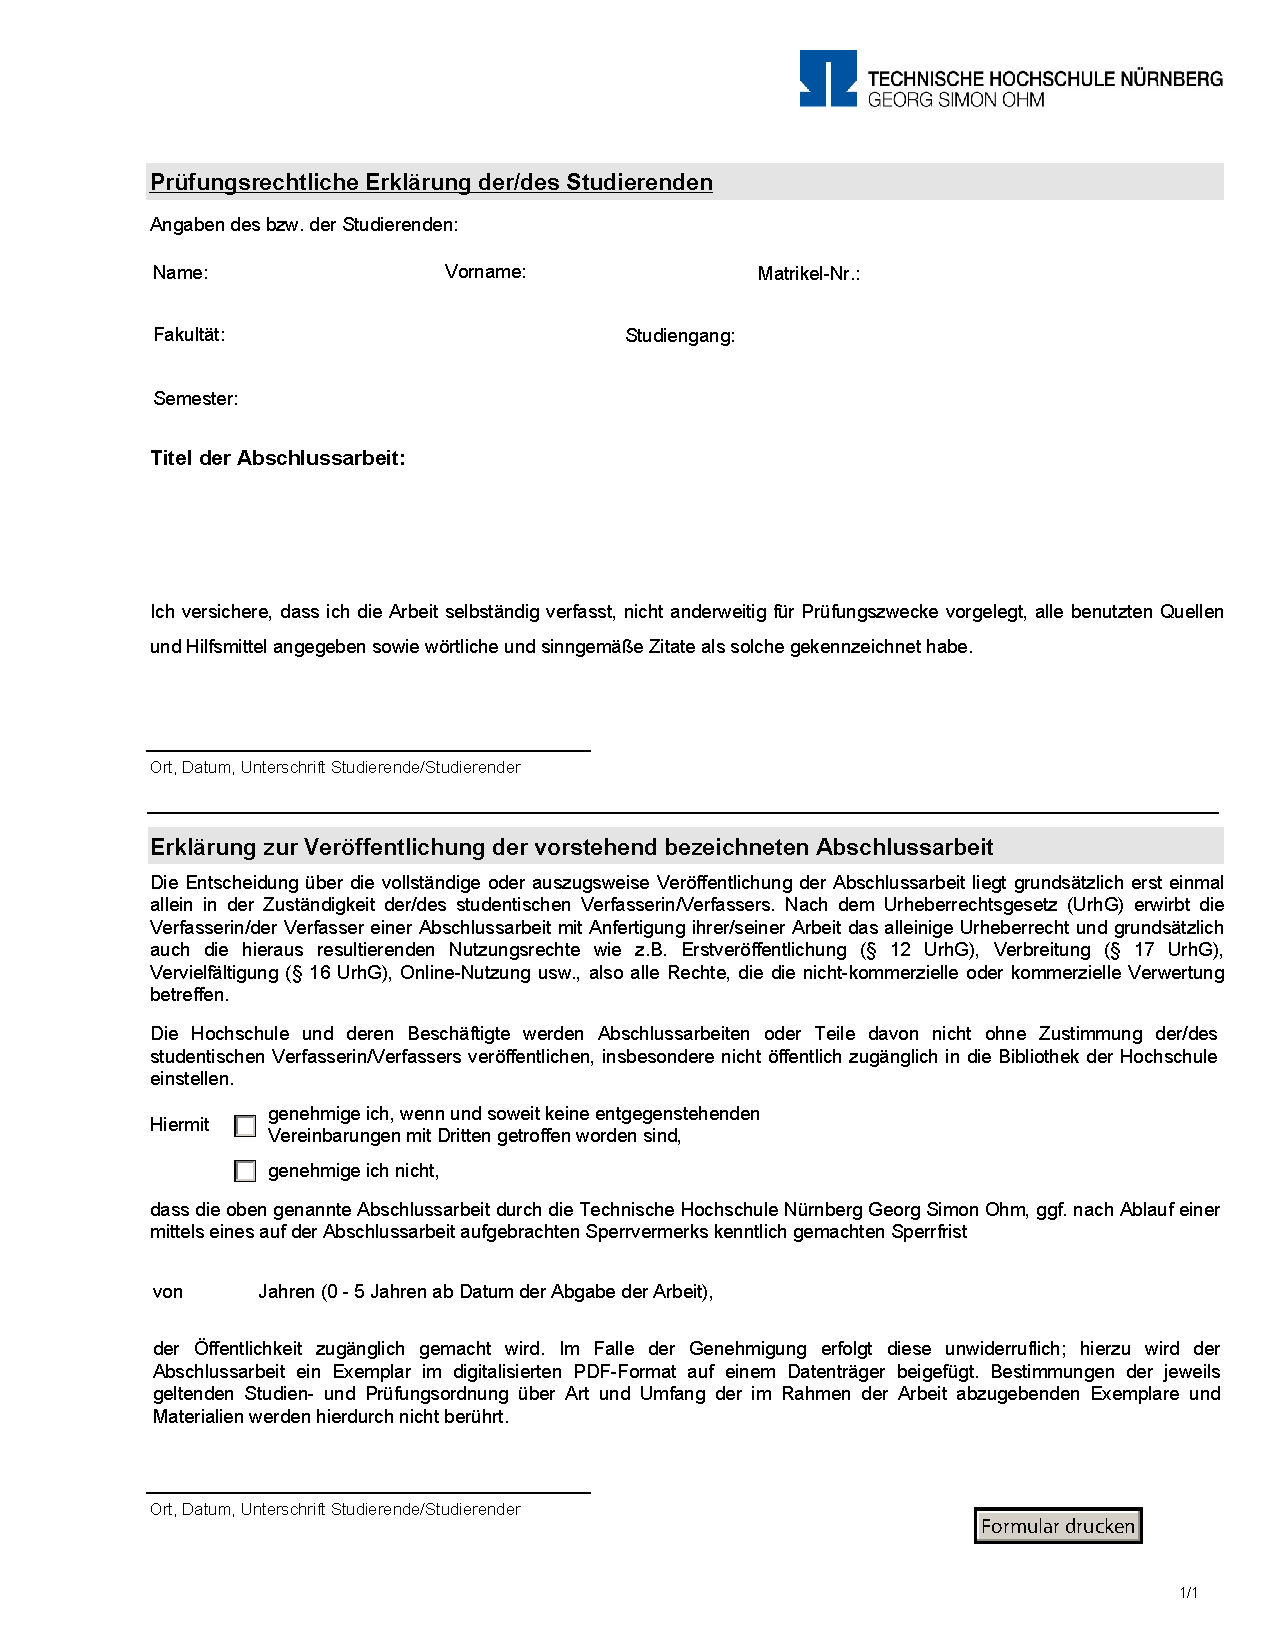
\includepdf{SB_0050_FO_Pruefungsrechtliche_Erklaerung_und_Erklaerung_zur_Veroeffentlichung_der_Abschlussarbeit_public.pdf}
\let\cleardoublepage\clearpage
% !TeX spellcheck = en_GB
% !TeX encoding = UTF-8

\section*{Abstract}
\label{sec:abstract}

Nowadays, the decisions made by \gls{dl} Algorithms influence our everyday life. Since the Discussion around the "Directive on Copyright in the EU Digital Single Market" had started, more and more people are interested in the decisions which are made by algorithms. In the following, this thesis provides an theoretical introduction about \gls{ml}, \gls{dl} and \gls{xai}. Moreover, a prototype gives a realistic insight into how \gls{dl} and \gls{xai} can be implemented within a Jupyter Notebook. Finally, the achieved results get evaluated and generalized among the topics of \gls{ul}.

\section*{Preface I}
My work at the Siemens AG had given me tremendous insight into the business analytics field. But since my interested is going more into the statistics Field, I was highly motivated to work on topics related to  \gls{ml} and  \gls{dl}. In the next few years, I think of a position in the Data Science Field, and so I committed myself to a final year project which covers this field as well. The \gls{xai} area made me even more curious to find out what we can learn from machine learning algorithms. To work on this was a tough challenge,  but at least it was a useful insight into scientific writing. 

\section*{Preface II}

The first time I came into contact with Machine Learning was through an IT project. The intention was to develop a self-driving car, controlled by a deep neural network. The whole project was very challenging, but I had a lot of fun, and my motivation was even higher. My motivation was immediately put a rough test in my exchange semester. In Hong Kong, I focused on machine learning during the entire semester.  Mathematical proofs that were required to can pass one of the courses were an extremely challenging task. Mainly because of lacking prior knowledge of statistics, I had to work twice as hard. During the semester,  I was able to close the gaps, master the tasks and finally did an excellent job at the programming part. This experience has strengthened my wish to concentrate further in this direction, and so I was highly motived to put everything that I have learned into my final year project. Since then, I have learned a lot and even if the work was not as perfect as it could it helped me a lot particularly since I am participating in the computer science master program with a focus on data science. I am sure there is more to learn. So,  I think this thesis was a tiny step in my life long learning journey.
\tableofcontents
\let\cleardoublepage\clearpage
\mainmatter
\let\cleardoublepage\clearpage
% !TeX spellcheck = en_GB
\chapter{Introduction}
\label{ch:Introduction}
\epigraph{"Most times, the way isn’t clear, but you want to start anyway. It is in starting with the first step that other steps become clearer."}{― Israelmore Ayivor, Leaders' Frontpage: Leadership Insights from 21 Martin Luther King Jr. Thoughts}
\section{Upload Filter in the public discussion}
\label{sec:directiveCopyrightUploadFilters}

The "Directive on Copyright in the EU Digital Single Market", which came into force on the 7th of June in 2019,  introduced a requirement for an automated \gls{ul}. The discussion refers to Article 17 (previously Article 13) because it forces content-sharing services such as Facebook, Google and YouTube to be responsible for copyright violations. From this point on, it is no longer possible to check contents manually \cite{Emmawoollacott2019}.\\

In Figure \ref{fig:00_protest_gegen_upload_filter} you can see Protesters in Berlin. For them, the fear of an \gls{ul} is real. They are concerned that these filters can harm their business as small content creators or their freedom of speech.

\begin{figure}[!htp]
	\centering
	\includegraphics[width=0.8\linewidth]{photo/00_protest_gegen_upload_filter.jpeg}
	\caption{In Berlin, opponents of the copyright directive are protesting. They fear that Article 13 will lead to upload filters, which they see as a danger considering different aspects \cite{Protestg81:online}.}
	\label{fig:00_protest_gegen_upload_filter}
\end{figure}

Different parties, organizations and scientists are arguing for and against the copyright directive. For example, the Christian Democratic Union (CDU)  and its representative at the European Parliament Axel Foss support the directive.  He said that it protects the freedom of expression on the internet and a diverse media landscape \cite{Europarl2017}. Critics as Julia Reda from th e Pirate Party  (also a member of the European Parliament) denies this statement. She described it as a change into a dark future for internet freedom, when upload filters would check every content automatically \cite{Emmawoollacott2019}.\\

More precisely, she assumes that technology does not know the nuances of particular copyright law yet. And even more, she fears that small content creators are not able to interpret the decisions of the upload filters \cite{Reda2019}. Dr Gallwitz is an associate professor at the Technical University of Nuremberg where he is researching in the field of pattern recognition. He criticized that there is no smart software that could recognize quotations from other sources \cite{Gallwitz2019}.\\

Instead of using smart software, a real-world \gls{ul} is realized through fingerprinting. This technique allows comparing blocked content with the latest user-generated content. The hardware requirements which are needed to compare the contents are proportionally small. Less high hardware requirements are one of the reasons why most companies still use older techniques (e.g. hash values), even they can build smarter \gls{ml} models \cite{Spoerri2019} \cite{Wagner1983}.\\

The Microsoft software Photo-DNA identifies child pornography with the fingerprinting method, e.g. if an image in Microsoft's database is marked as pornographic. That means YouTube can detect when someone wants to upload such an image to the platform \cite{Microsoft2013}. The Software Content ID uses the same technique to identify copyright offences. It is used and developed by YouTube. That shows how Technique Companies are responsible for which method is used. Even scientific research has shown that different approaches are performing better, the companies have to see this decision from a business point of view \cite{YouTube2010}.\\

Using \gls{ml} models as upload filters in the future could be possible, but among this usage are many problems. One of them is to get labelled data (necessary to train a model) which can detect patterns. Another problem is to define the patterns or the labels itself \cite{WaltermannHubertus2019}. Labels are categories which you could assign to an image \cite{Goodfellow-et-al-2016} e. g. attach the label cat to an image with a cat. In the case of copyright violations or offensive content, we block any item that has labels with copyright content. A machine learning algorithm which can detect all assaulting labels alone must be complex because the complexity from machine learning algorithms is increasing with increasing input features and an increasing amount of expected outputs \cite{Yao2017}. In machine learning terms, a feature is any input we can put into a machine learning algorithm, e.g. an image with 32 x 32 pixels has 1024 input features because every pixel counts as a single feature \cite{Goodfellow-et-al-2016}.

\section{Upload filters and Explainable Artificial Intelligence}
\label{sec:uploadFiltersXAI}

As mentioned in \hyperref[sec:directiveCopyrightUploadFilters]{the introduction to the Directive on EU Copyright and Upload Filters (\ref{sec:directiveCopyrightUploadFilters})}, a \gls{mla}, used to detect copyright infringements would be too complex. Joel Dudley, director of the Institute for Next-Generation Healthcare at the Ichan School of Medicine, said: "We can build these models, but we don't know how they work." \cite{Knight2019}. His statement was part of an interview with the journalist Will Knight from MIT's Technology Review about Explainable Artificial Intelligence (XAI). A precise definition of what exactly \gls{xai} is does not exist. The global idea is that we use a \gls{mla}to make decisions which must be in natural language. For example, if we use an image as an input for a \gls{mla}, the task would be to label the images with a label for cancer or no cancer. A doctor who wants to use this information could be interested in the question of why the algorithm, predicts a cretin label for this image. \cite{SamekWojciech2017}.\\

Apart from the Technology Review, newspapers like The New York Times, Financial Times and The Register have also reported that an \gls{xai} is necessary an \gls{mla} is used for an automatic decision making \cite{Kuang2017} \cite{Robinson2017} \cite{Waters2017}. David Gunning explains in his research project about \gls{xai} that \gls{ml} can bring a huge benefit to the transportation sector, as well as to the finance , security , legal , medicine and military sector. Gunning claims that algorithms are limited, because they can not explain their actions and decisions to users in an understandable way. He assumes \gls{xai} will be essential if users want to understand, trust, and effectively manage this incoming new \gls{ml} Algorithms\cite{Gunning2019}. Figure \ref{fig:01_upload_filiter_example} shows an example of how transparent \gls{ul} can be applied to uploaded images. Even this look not intuitive for a non-technical user, if we build an \gls{ul} with \gls{dl} methods, it has to be an \gls{xai} \cite{WaltermannHubertus2019}. Otherwise, there will be no explanation of how the decision from an \gls{ul} was made.\\

\begin{figure}[!htp]
	\centering
	\includegraphics[width=0.9\linewidth]{photo/01_upload_filiter_example.png}
	\caption{Example of how transparent \gls{ul} can be applied to uploaded images \cite{Visualiz76:online}}
	\label{fig:01_upload_filiter_example}
\end{figure}

\section{The Goal of this Thesis}
\label{sec:goal}

Even automatic image recognition in \gls{xai} with \gls{dl} procedures is just a research topic, it is important to evaluate how we could generate comprehensible decisions (XAI). So, the main objective is to find an answer to the following question:
\begin{quote}\textit{"How can automatic image recognition be implemented in such a way that the resulting decisions are transparent?"} \end{quote}
For this purpose, I would like to develop an algorithm which should be able to recognize patterns on images (automatic image recognition) automatically. If a pattern is recognized by the algorithm, it should assign a label to the image.  In the pre-field, I define which markings correspond to appropriate content and which to inappropriate content. This way, the algorithm should finally decide which images are appropriate or inappropriate according to the criteria I defined before (\gls{ul}).

Afterwards, the results of the algorithm are presented in such a way that the decisions become transparent (\gls{xai}). What transparent actually means is hard to tell at this point of my thesis, because it depends on the algorithms and techniques, which are used to implement the filter. Anyway to make things more clear, transparent could explained as the following:

\begin{quote}
\textit{Imagine a social media platform like Instagram, where everybody could share its images. If someone shares an image and it is getting blocked by a filter (e.g. because of copyright violation), the user should be able to understand why the decision would be made. There could be an automatically generated text, which says that the algorithm had detected a copyright issue and it highlights specific parts in the blocked image. The highlighted details should tell the user why the algorithm came to decision (content is protected by copyright law).
}

\end{quote}

In contrast to my example, an application in real life would be much more complicated. First, in such a real-world application, there is a much more extensive range of labels that the algorithm could set. Second, it is not only possible to upload images, but also text and sound which would have to be checked. Therefore my example application is only a prototype. Anyway, the question is asked on top of this section will be answered anyways. At least from a theoretical perspective. In the end, I would like to use my prototype to transfer the knowledge gained to a more general scenario.

\section{Thesis Structure}
\label{sec:structure}

A brief \hyperref[ch:Introduction]{Introduction (\ref{ch:Introduction})} about the two main terms \gls{ul} and \gls{xai} is already addressed in the previous introduction section. Preface I and II is about the motivation for this thesis and about the prior knowledge which in order to work on this task. The \hyperref[ch:theory]{"Requirement Chapter"(\ref{ch:theory}} focuses on details which are necessary to answer the question which is given at \hyperref[sec:goal]{the Goal of this Thesis (\ref{sec:goal})}. The \hyperref[ch:requirements]{"Requirements"(\ref{ch:requirements}} section defines properties and demands of a \gls{ul} prototype which makes transparent decisions with the help of \gls{dl} and \gls{xai} methods. The next two chapters (\hyperref[ch:functional_specifications]{introduction (\ref{ch:functional_specifications})},(\hyperref[ch:it_specifications]{introduction (\ref{ch:it_specifications})}, are presenting an analytical approach o how such a prototype can be implemented. The next chapters are applying the answers to a broader use case scenario like described in section \hyperref[sec:goal]{"The Goal of this Thesis" (\ref{sec:goal})}. It starts with an evaluation followed by a generalization and ends with a summary. Before the work on this thesis has actually started, to finish a structured plan in the methodological table (Figure \ref{fig:02_methodological_table}.) was mandatory. Here it is presented in a translated and shortened version. Here can be seen a detailed explanation of the thesis structure. 

\begin{figure}[htp]
\centering
    \includegraphics[max size={\textheight}{\textwidth},angle=90]{photo/02_methodological_table.pdf}%<---angle here
    \caption{Methodological table  which was prepared in the run-up to the bachelor thesis in cooperation with the assesor Dr Prof Alfred Holl.}
    \label{fig:02_methodological_table}
\end{figure}

\section{Related Work}

Katharina Blandina Weitz wrote in her master thesis "Applying Explainable Artificial Intelligence for Deep Learning Networks to Decode Facial Expressions of Pain and Emotions" about programmes used in hospitals, which detect pain in facial expressions. According to her, this software should use deep learning to support human practitioners. Towards her thesis, Ms Weitz found out that these deep learning methods work well in recognising pain in human facial expressions, but they are hard to interpret. From her abstract, you can learn that XAI does not depend on a specific data set that was used to perform a machine learning task. Rather, according to their statement, the methods can be applied to any dataset that was previously used for a task that was processed by deep learning \cite{Weitz2018}. As described in \hyperref[sec:goal]{the Goal of this Thesis (\ref{sec:goal})} the contexted will be changed among this thesis.\\

\begin{figure}[!htp]
	\centering
	\includegraphics[width=0.6\linewidth]{photo/03_DARPA_XAI_Project.png}
	\caption{Explainable Artificial Intelligence Concept from the Defense Advanced Research Projects Agency \cite{Robinson2017}}
	\label{fig:03_DARPA_XAI_Project}
\end{figure}

The Defence Advanced Research Projects Agency (DARPA)is an agency of the United States Department of Defence. They focus on the development of emerging technologies that the military could use. Because both the number of applications and the complexity of \gls{ml} models have increased, a project has been started to specialize in \gls{xai}. It aims for more transparent models while maintaining a high level of prediction accuracy. Furthermore, the program wants to enable human users to understand, appropriately trust, effectively manage the output a \gls{mla} \cite{Robinson2017}. Figure \ref{fig:03_DARPA_XAI_Project} shows how the Defense Advanced Research Projects Agency presents its projects as a concept. As I have also described in \hyperref[sec:goal]{the Goal of this Thesis (\ref{sec:goal})}, the concept wants to move away from a model that human users cannot understand towards to a more transparent model. 

There are more scientific papers on \glossary{xai}, but a complete bibliography is unfortunately not possible within this work.\\

\let\cleardoublepage\clearpage
% !TeX spellcheck = en_GB
% !TeX encoding = UTF-8
\chapter{Background and Theory}
\label{ch:theory}
\epigraph{"Math is like water. It has a lot of difficult theories, of course, but its basic logic is very simple."}{- Haruki Murakami, IQ84}

This chapter is a summary of all fundamental aspects of \gls{ml}. More specifically, the crucial elements for an understanding of the prototype-functionality, which is presented later on. First of all, the historical development of \gls{ml} will be covered briefly. As soon as the reader has an understanding of the historical development of \gls{ml}, its categories will be discussed. Therefore, not every detail is covered. Only aspects and algorithms of \gls{ml} which are relevant in order to talk about the topic of this thesis. In the final part of this chapter, two different approaches of \gls{xai} are introduced. Furthermore, a specific kind 
\gls{xai} implementation is mentioned, such that the reader can understand how predictions can be made transparent.

\section{History of Machine Learning}
\label{sec:history}

An example of \Gls{ml} would be to take a lot of images and try to recognize cats (patterns) on them. The \Gls{mla} would be able to predict - for new images in the future - whether it is a cat or not. In this example, \gls{ml} can be seen as

\begin{quote}\textit{"[...] a set of methods which can automatically detect patterns in data, and then use the uncovered patterns to predict future data or to perform other kinds of decision making under uncertainty" \cite[p. 1]{Murphy2012}.} \end{quote}

But there is more than one definition which describes \gls{ml}. Arthur Samuel was the first researcher who used this term and defined it as "Machine Learning is a field of study that gives computers the ability to learn without being explicitly programmed" \cite{Samuel1959SomeSI}. The computer scientist Mitchel provided a more formal definition of \gls{ml}, which is quoted in hundreds of papers\footnote{998 results on google scholar while searching for the original meaning from Mitchel (date: 24 Jan 2020)}. In his book from 1997, he says "A computer program is said to learn from experience E concerning some class of tasks T and performance measure P, if its performance at tasks in T, as measured by P, improves with experience E" \cite{Mitchell97}.\\

\begin{figure}[!htp]
	\centering
	\fbox{\includegraphics[width=1\linewidth]{photo/04_history_of_machine_learning}}
	\caption{Determining critical technologies within the domains of \Gls{ai} (extended representation by Dmitri Gross according to a presentation from Michael Copeland) \cite{Gross2017} \cite{COPELAND2017}}
	\label{fig:04_history_of_machine_learning}
\end{figure}

According to the science magazine, the most influential computer scientist, in the field of pattern recognition, Michael Jordan wants to give another modern definition. His objective was to give a neutral statement, which defines the word \gls{ai}. He says:

\begin{quote}
	\textit{"It is one of today's rapidly growing technical fields, lying at the intersection of computer science and statistics, and at the core of artificial intelligence and data science" \cite{Bohannon2016} \cite{Jordan255}}
\end{quote}

Furthermore, with this definition, Jordan wants to connect the terms of \gls{ml} and statistics. In his opinion, these two terms are the essential components of \Gls{ai} \cite{MichaelJordan2018}. Figure \ref{fig:04_history_of_machine_learning} shows how machine learning has changed over the last decades. It shows that machine learning became popular in the eighties, as a result of the increasing use of personal computers (PC). Furthermore, you can see deep learning - which is one of the crucial parts of my thesis - gained on popularity until 2010, caused by the development of more powerful \Gls{gpu} (GPU). Besides Figure \ref{fig:04_history_of_machine_learning} is criticized as well. Mainly because of the unclear definitions terminology which is used in it. Anyways it can be used to get an overview of the historical evolution of the field. 

\begin{figure}[htp]
	\centering
	\fbox{\includegraphics[width=0.4\linewidth]{photo/05_deep_learning_sucess_with_alpha_go.jpeg}}
	\caption{The Netflix documentary Alphago is part of the hype around \gls{dl} Methods. Critics claim until the problem of transparency is not solved this results are not crucial because those models can not be used in a real-world application \cite{Thetruec1:online}}
	\label{fig:05_deep_learning_sucess_with_alpha_go}
\end{figure}

Alpha Go, which is developed by the Google Research Laboratory, is a good example of the popularity of \gls{dl} Methods. It shows how an enormous amount of time and hardware resources can lead to success as the artificial player has been the world ranked number one in the board game go. But this success is criticized as well, because it is not a real-world application and gots pushed by a Netflix Documentary, Scientist Claim that it is just an overhyped topic as long as the models could not be explained (Figure \ref{fig:05_deep_learning_sucess_with_alpha_go}).

\section{Suprvised Machine Learning for Upload Filters}
\label{sec:supervised_learning}
By doing the following steps, a \Gls{cf} (Definition \ref{def:cost_function}) will be optimized to get a prediction on unseen data, as defined by Mitchel (Section \ref{sec:history}). An example application is an \gls{ul} which determines if a dog or a cat is on an image:

\begin{enumerate}
	\itemsep-0.8em 
	\item Eliminate empty entries and statistically irrelevant data (e.g. duplicates) 
	\item Put input data in the required form (defined the form of implementation)
	\item Split the Data into a test and a training set (to test on unseen data)
	\item Initialize the parameters of the model
	\item Learn the parameters for the model by minimizing the \gls{cf}(Definition \ref{def:cost_function})
	\item Use the learned parameters to make predictions (Definition \ref{def:mapping_function}))
	\item Test the ability of the model to predict unseen data correctly
\end{enumerate}

In the following, these steps are described while focusing on the details of the current step. The example of an Instagram Upload filter is a \Gls{clt} which can be solved by a \Gls{sla}. It is designed to learn by example (cat images) \cite[p. 3 - 4]{Murphy2012}. As can be seen in Figure \ref{fig:06_example_dog_vs_cat_dataset}, examples of cats and suitable counterexamples are assumed to be given before we start to design an \Gls{sla}.\\\\

\begin{figure}[htp]
	\fbox{\includegraphics[width=1\linewidth]{photo/06_example_dog_vs_cat_dataset}}
	\caption{Images of detected cats, examples sampled from the from the "ImaegNet" data set\cite{Building13:online}}
	\label{fig:06_example_dog_vs_cat_dataset}
\end{figure}

The name "\Gls{sl}" comes from the idea that training this type of algorithm is like having a supervisor which observes the whole learning process, e.g. recognize cats on images after having seen enough examples and counterexamples. At the same time, someone leads the algorithm to the correct result \cite[p. 103]{Goodfellow-et-al-2016} \cite[p. 3]{Murphy2012}. Technically spoken, these input data is called \gls{td}. They consist of input data (for example, values that represent an image) and output data (for example, the class which an image belongs to). During training, the algorithm will search for patterns in the input data that correlate with the desired outputs. After training, the supervised learning algorithm will take in new unseen inputs (cats, no cats or both). Afterwards, the algorithm determines which labels, are used to classify the original inputs, based on prior training data. Such an algorithm can be expressed as follows \cite[p. 3]{Murphy2012}:

\begin{definition}[label=def:mapping_function]{Mapping Function}
	\begin{align*}
	f(X) = \hat{y}
	\end{align*}
	where \\\\
	f() = mapping function e.g. assigns the label cat to a cat picture\\
	X   =  (several) input values e.g. images with cats\\
	\( \hat{y}\) = predicted output e.g. a label with cat or no cat\\
\end{definition}

Where \(\hat{y}\) is the predicted output, which is determined by a mapping function \(f\) that assigns a label to a single value or a set of multiple-input values donated by \(X\), the function connects an input (features) to a predicted output (probability). The logic behind this function is also called machine learning model \cite[p. 3]{Murphy2012}.\\

Before \gls{mla} (model) which detects cats on images gets trained, the \Gls{td} has to be prepared. This step is called \Gls{pp}. Training data consists of inputs paired with the correct outputs \cite{brownlee2019deep}. For example, the inputs are the samples of cat images, where the outputs are the right labels of our examples. When talking about the training of a \gls{mla} (Model), the optimization of a function is always meant by that. Further, the function to be optimized is the mapping function which assigns an output value to the given input. Therefore the parameters of the function will be optimized during the training process, such that the output values match the actual output values as closely as possible. In other words, such that the real values as close as possible to the predicted values  (Definition \ref{def:cost_function}). Usually, that is an optimization problem and is solved with different techniques. The technique also determines the required form of the input and output data (Step 2). If we used a \Gls{lr} to classify cats, a structure as can be seen in Definition \ref{def:structure_for_linear_logistic_regression} is necessary. \gls{lr} is a model which is applied to determine the probability of a certain class or event exists such as pass/fail, win/lose, alive/dead or healthy/sick. It can be extended to predict several classes of events such as determining whether an image contains a cat, dog, lion, etc.

\begin{definition}[label=def:structure_for_linear_logistic_regression]{required input format for a machine learning program with logical regression}
	\begin{align*}
	& X \in \mathbb{R}^{n_{x}\times m}  \\
	& y \in \mathbb{R}^{m}
	\end{align*}
	where \\\\
	\( X \)X = an input matrix e.g. each column represents the values of an (cat) images\\
	Y = a single row matrix e.g. each column holds a binary value (yes/ no)\\
	\( n_{x} \) = number of values which represents one example e.g. pixels of an image \\
	m = number of examples e.g. (cat) images \\
	\( \mathbb{R} \) = all values are in real number space \\
\end{definition}

A pixel image of a cat, as you can see on the left-hand side in Figure \ref{fig:07_image_vector_representation.png}, is represented as three matrices (Figure \ref{fig:07_image_vector_representation.png}, centre). With the help of mathematical functions from the field of linear algebra, the images are transformed from the matrix form into a vector form (Figure \ref{fig:07_image_vector_representation.png}, right) \cite[p. 276]{brownlee2019deep}. Even if it is not necessary, it is recommended to normalize the values. Otherwise, the calculations could become very slow and very memory intensive. \cite[p. 57]{Goodfellow-et-al-2016}.

\begin{figure}[htp]
	\fbox{\includegraphics[width=1\linewidth]{photo/07_image_vector_representation.png}}
	\caption{At the beginning a picture is represented by three matrices. Each for one colour channel (red, green and blue). After transforming it with linear algebra we get a vector.}
	\label{fig:07_image_vector_representation.png}
\end{figure}

Because we want to optimize the \gls{cf} (Definition \ref{def:cost_function}) for many examples, instead of just one, we store the input in a matrix (Definition \ref{def:structure_for_linear_logistic_regression}). After transforming a picture, we get a vector, so it is mandatory to store every single vector in the column of a matrix. Matrix representations are one of the reasons why machine learning algorithms are much more efficient because nowadays, memory is cheaper than computing power. Without matrix multiplication, more loops would be needed. Loops, on the other hand, require a relatively large amount of computing power, especially for extensive data. Matrix multiplication requires a lot of memory but requires fewer loops and therefore, less computing power. Due to the extreme amounts of data that are processed during the calculation of machine learning algorithms, these effects are multiplied by each other, which makes an efficient computation even more important \cite{AndrewNG}.\\

The next step in designing a \Gls{sla}(after the preprocessing is done) is to create a specific function which can be optimized. At first, a linear function which looks like the following is used:

\begin{definition}[label=lf]{A Linear Function as a vector and matrix representation to compute multiple input values at once}
	\begin{align*}
	z = W X + b
	\end{align*}
	where \\\\
	z = Results of the linear function (one for each example)\\
	W = A matrix with parameters assigned to every row of the input matrix X\\
	X = Matrix as a result of the preprocessing \\
	b = Intercept added in a linear equation called \Gls{bias} parameter.\\
\end{definition}

The output values of the linear function can then be passed to a \Gls{sf}. Every function which is used after calculating the linear function itself is an so-called \Gls{af}. They are mathematical equations to determine the output of a neural network. An \Gls{af} can be used for different tasks. So the \gls{sf} (Definition \ref{def:sf}) is one specific example which maps a value between 0 and 1 to each output. In such a way, that this value can be interpreted as a probability (Definition \ref{def:sf}). Finally, a label can be assigned to the input by using a rule-based approach. For example, it could be the case that if the probability is greater than 50\% that a certain case will occur, a positive label will also be assigned (the probability that a cat is on the image is greater than 50\%, then the image has the label cat).\\

\begin{definition}[label=def:sf]{Sigmoid Function e.g. for using it to get probabilities}
	\begin{align*}
	\hat{y} = sigmoid(z)
	\end{align*}
	where \\\\
	z = The results of the linear function (one for each example)\\
	\( \hat{y}\) = Calculated labels (one for each example) \\
\end{definition}

The next step for the Instagram Upload Filter is to get a criteria, which we can use to optimize the parameters. In other words to quantify the success of our training process. In order to get such a criteria a so-called error value is formed. This is calculated from the actual label (\(y\) )and the predicted label (\( \hat{y} \)). How exactly this calculation is done is determined by the loss function. For example the loss function could be defined by the cross-entropy function \(\mathcal{L}\), which compares the given values with the calculated values. Every function in machine learning that could be used to compute such an error would be called \Gls{lf}. Finally, all error values of the individual examples are summed up and divided by the total number of examples (images). This way, we get an error function \(\mathcal{J}\) which maps a single value to all errors. This error function can be optimized during the training process so that we get parameters (\(\mathcal{W} \) and b) of the function which leads to a global minimum of the function. While in the first step, the so-called \gls{fp}, the error values and calculations are performed, in the second step the weights of the function will be optimized. This step uses the chain rule to form the gradient of the weights and adjust them according to this gradient. In the literature, the second step is commonly called \gls{bp}. I will go into this procedure in more detail in section  \hyperref[sec:gd]{Gradient Decent and the Gradient (\ref{sec:gd})}. Because it shows the overall cost in \Gls{ml} Literature, the function which sums up every loss of each input is name \Gls{cf}:

\begin{definition}[label=def:cost_function]{Cost Function which can be optimized}
	\begin{align*}
	\mathcal{J} = \frac{1}{m} \sum_{i=1}^m \mathcal{L}(\hat{y}^{(i)}, y^{(i)})
	\end{align*}
	where \\\\
	m = Number of examples e.g. number of cat and no cat images \\
	\(\mathcal{L}\) = Cross-Entropy function \\
	\(\hat{y}\textsuperscript{i}\) = Calculated label for the \(i\textsuperscript{th} \) example\\
	\(y\textsuperscript{i}\)     = Correct label for the \(i\textsuperscript{th} \)  example\\
	\(    \mathcal{J} \) = Cost Function which can be optimized s. t. it is at its global minimum
\end{definition}

The \Gls{cf} should not be optimized as close as possible to the training data. A function which would fit perfectly is called over-fitted. 

Overfitting means models perform well on the training data but don’t generalize well for new data. It happens when the model is too complex relative to the amount and noisiness of the training data. So, how do we know the parameters are overfitted? If a test against the training set gets excellent results but, a test against the test set has very low accuracy, t model is likely overfitted. So, it's time to take corrective measure \cite[p. 110]{Goodfellow-et-al-2016}. Anyway, the goal of supervised learning as in the Instagram Upload Filter is to achieve high performance on unseen data. To do that the data has to be divided into a test and a training set. The training set is used like described before (preprocessing the data and approximate the cost function to its global minimum). In contrast, the test data set would only be preprocessed and then used to make predictions about unseen cat images. So it is possible to test the neural network of its ability to predict unseen data (\hyperref[sec:history]{History of Machine Learning (\ref{sec:history})}).\\\\

In other words, every step is necessary to train a machine-learning algorithm to predict if it is a cat or not. In figure \ref{fig:08_process_of_pretictions_for_a_cat_image} where

\begin{itemize}
	\item \(\boldsymbol{x\textsubscript{x}} \) is \(x\textsuperscript{th}\) pixel of an image representation,
	\item \(\boldsymbol{W\textsubscript{x}}\) is \(x\textsuperscript{th}\) parameter assigned to each pixel of\(x\textsuperscript{th}\),
	\item \textbf{W X + b} is  the linear function which computes a first output and
	\item \(\boldsymbol{\sigma}\) is the sigmoid function
\end{itemize}

is the process of predicting an \(64\times64 \) image visualized.

\begin{figure}[htp]
	\fbox{\includegraphics[width=1\linewidth]{photo/08_process_of_pretictions_for_a_cat_image.png}}
	\caption{The image visualizes the whole process of using an image (1) and putting this into a single neuron (4). First, the neuron calculates a linear function and uses the result as input to a sigmoid function (becomes an interpretable value between zero and one). The network can make a prediction (5) while using a decision boundary (e.g. if the probability is higher as 0.5 that it is a cat) if the forecast is not correct, the parameters of the function (2, 3) getting adjusted as long as the function is optimized. Finally, we hat an approximation that fits (as close as possible) to all training examples.}
	\label{fig:08_process_of_pretictions_for_a_cat_image}
\end{figure}

An algorithm that works like this can be considered as simple neural network \cite{Britz2015}. The term neural came from the fact that at first scientists tried to recreate the functionality of neurons in the human brain. Besides the early beginning, neural networks haven't much in common with the brain because actually, it seems the brain is much more complicated as it seems before \cite{Kriesel2007NeuralNetworks}. However, it is called a network because usually different neurons working together. In the simple scenario from Figure \ref{fig:08_process_of_pretictions_for_a_cat_image} we had just one neuron (Figure \ref{fig:09_example_of_a_single_neuron})

\begin{figure}[htp]
	\centering
	\fbox{\includegraphics[width=0.4\linewidth]{photo/09_example_of_a_single_neuron}}
	\caption{An Example for a single neuron. First, a linear the output will be calculated by a simple linear function with the parameters \(W\) and \(b\). Afterwards the output will be normalized to get probabilities (values between 0 and 1).}
	\label{fig:09_example_of_a_single_neuron}
\end{figure}

For the Instagram Upload Filter, such a \Gls{nn}\footnote{The achieved accuracy is not always precisely the same, because the local minimum is reached during optimization instead of the global minimum. In practice, this change is hardly relevant. Besides, the results can differ depending on the implementation. The results presented here were obtained with the programming language Python using frameworks from the field of data science.} achieves a test accuracy of about 70\% (Listing \ref{lst:acc}).\\\\

\begin{lstlisting}[captionpos=b,label={lst:acc},language=Python, caption=Test accuracy is 70\% after iteration 2000 times and using 209 examples with 12287 features (\(64\times64 \) pixels). This is not state of the art but very good if considering that this is a linear classifier on a high dimensional feature space.]
Cost after iteration 0: 0.693147
Cost after iteration 1000: 0.214820
Cost after iteration 1100: 0.203078
Cost after iteration 1200: 0.192544
Cost after iteration 1300: 0.183033
Cost after iteration 1400: 0.174399
Cost after iteration 1500: 0.166521
Cost after iteration 1600: 0.159305
Cost after iteration 1700: 0.152667
Cost after iteration 1800: 0.146542
Cost after iteration 1900: 0.140872
train accuracy: 99.04306220095694 %
test accuracy: 70.0 %
\end{lstlisting}

It is crucial to achieve a higher accuracy before creating a transparent neural network which is easy to understand. To introduce more precise methods is the goal of the next section.

\subsection{Deep Learning Neural Networks}
\label{subsec:deep_learning}
Instead of just using one neuron to predict if an image shows a cat, the \Gls{nn} can look like in Figure \ref{fig:10_process_of_pretictions_for_a_cat_image_two_layers}, where

\begin{itemize}
	\item \(\boldsymbol{x\textsubscript{x}}\) is the \(x\textsubscript{th}\) pixel of an image representation,
	\item \(\boldsymbol{a\textsubscript{[1]}}\) is calculated input values from the first layer,
	\item \(\boldsymbol{W\textsubscript{[1]}}\) is the parameters assigned to each pixel of \( x\textsubscript{x}\),
	\item \(\boldsymbol{W\textsubscript{[2]}}\) is the parameters assigned to each input  \(a\textsubscript{[1]}\textsubscript{n}\) input, calculated by layer one
	\item \textbf{W X + b} is the linear function which computes a first output and
	\item \(\boldsymbol{\sigma}\) is the sigmoid function,
\end{itemize}

\begin{figure}[htp]
	\centering
	\fbox{\includegraphics[width=0.8\linewidth]{photo/10_process_of_pretictions_for_a_cat_image_two_layers.png}}
	\caption{The picture visualizes the whole process of using an image (1) and putting this into two neurons (1,2). The first calculates a linear function and put the result into a  function so that it can be forwarded normalized to the second neuron. The next takes the values and calculates (as before) the result of a linear function which would be made interpretable while using the sigmoid function (between zero and 1). Last but not least, the result can be interpreted so that the network can make a prediction (5). If the forecast is not correct, the parameters of the function (2, 3, 4) getting adjusted. It will be adjusted (fitted) as long as the function is optimized to match as best as possible to all training examples.}
	\label{fig:10_process_of_pretictions_for_a_cat_image_two_layers}
\end{figure}

shows how the same network as before would look like if we would use two neurons  (1, 3) in two layers (4,5). On the one hand, more neurons resulting in an increasing amount of parameters which the algorithm has to optimize \cite[p. 21]{Goodfellow-et-al-2016}. So, for example, to find a global minimum for a \Gls{cf} in our Instagram Upload Filter example, it would take significantly more time and requires more cat images. But on the other hand (if correctly implemented) a neural network with more neurons and multiply layers would outstand a neural network with just one neuron by far. Listing \ref{lst:acc2l} shows that the algorithm detects up to 80\% of the pictures (if it shows a cat example or not). So, the deep neuronal network, compared with a single layer neural network, has increased by 10\%.

As I mentioned before, the results could be much better if more examples were used as input data. The required time and computing capacity would be comparatively low with such an implementation. Nevertheless, I will use the algorithm with more input at this place, because the given amount is sufficient to present the mentioned advantages \cite[p.167]{Goodfellow-et-al-2016} \cite[p.995 - 997]{Murphy2012}.\\

In general, the term is related to the number of layers. Andrew Ng suggests that neural nets with more than one layer should be called deep \cite{AndrewNG}. Furthermore, every layer which is not the output and not the output layer itself would be called the hidden layer. Whereas the output layer counts to the total amount of layers, the input layer is usually not considered as a so-called layer. There is not an exact definition of what a layer exactly is. Most sources are excluding the input and including the output layer. Steps in which an activation function activates the neurons do not count as independent layers. They belong to the previous layer (to which the neuron also belongs which input this function receives to standardize it)\cite{AndrewNG} \cite{Kriesel2007NeuralNetworks} \cite{Goodfellow-et-al-2016}.\\

\begin{lstlisting}[captionpos=b,label={lst:acc2l}, float=tb,language=Python, caption=Test accuracy is 80\% after iteration 2400 times and using 209 examples with 12288 features (\(64\times64 \) pixels). This is not state of the art but very good if considering that this is an algorihm wich is not spezialised to recoginize images.]
...
Cost after iteration 1600: 0.148214
Cost after iteration 1700: 0.137775
Cost after iteration 1800: 0.129740
Cost after iteration 1900: 0.121225
Cost after iteration 2000: 0.113821
Cost after iteration 2100: 0.107839
Cost after iteration 2200: 0.102855
Cost after iteration 2300: 0.100897
Cost after iteration 2400: 0.092878
train accuracy: 98.5645933014 %
test accuracy: 80.0 %
\end{lstlisting} A problem with the neural network, which is not deep (introduced above) would be its capability of training with larger images. So, the network was built to recognize patterns on images with 1288 input features ((\( 64 \times 64\) pixels). Suppose the input is a (\( 300 \times 300\) RGB image, the first layer of the network has 100 neurons, and each one is fully connected (fully connected layer) to the input. Fully connected means that each neuron in the previous layer is connected to each node in the following layer.The number of parameters which the training process has to optimize would be calculated with the following formula \cite{Vasudev2019}\cite{DBLP:journals/corr/TraskGR15}.

\begin{definition}[label=cn]{Calculate the total number of neurons in a neuronal network}
	\begin{align*}
	& W\textsubscript{ff} = F\textsubscript{-1}\times F \\
	& B\textsubscript{ff} = F \\
	& P\textsubscript{ff} = W\textsubscript{ff}\times +  B\textsuperscript{ff}
	\end{align*}
	where \\\\
	\(W\textsubscript{ff}\) = Number of weights of a FC Layer which is connected to an FC Layer \\
	\(B\textsubscript{ff}\) = Number of biases of a FC Layer which is connected to an FC Layer \\
	\(P\textsubscript{ff}\) = Number of parameters of a FC Layer which is connected to an FC Layer \\
	F = Number of neurons in the FC Layer\\
	\(F\textsubscript{-1}\) = Number of neurons in the previous FC Layer
\end{definition}

In the equation above, \( F_{-1} \times F \)is the total number of weights (connections between layers) from neurons of the previous fully connected layer, to the neurons of the current fully connected layer. The total number of biases is the same as the number of neurons (F). So, for the example given above (\( 300 \times 300\) pixels, 100 Layers in the first hidden layer, RGB and fully connected) the calculation would look like this:\\\\
\begin{align*}
& W\textsubscript{ff} =  270.000 \times 100 = 27.000.000  \\
& B\textsubscript{ff} = 100 \\
& P\textsubscript{ff} = W\textsubscript{ff}\times +  B\textsubscript{ff} = 27.000.000 +100 =27.000.100    \\
& F: = 100 \\
& F\textsubscript{-1} = 270.000 \text{ (300 x 300 pixels x 3 colour channels})\\
\end{align*}
If the picture gets even bigger and the layers get more, you can't optimize the weights with standard hardware, because if you look at the calculation it becomes clear that the number of parameters is much bigger. As a guideline, there are about 14.000.000 parameters where it is still possible to train without special hardware (e.g. on your own computer). Everything above this is difficult to realize on a personal computer without any hardware adjustments.   Besides, the models could not predict in any case in a satisfactory time \cite{DBLP:journals/corr/TraskGR15}. Instead of the introduced neural network, there are particular implementations of deep neural networks that can calculate a forecast more efficiently.\\

The subject of the next section is to determine how to achieve excellent results in a reasonable time, even if the input image is greater than or equal to \( 300 \times 300\) pixels.

\subsection{Convolutional Neural Networks}
\label{subsec:cnn}

The most popular deep learning models leveraged for computer vision problems are convolutional neural networks. To present the \Gls{cnn} (which will be made transparent), the example given at the beginning of this chapter will be changed. Instead of cats, the network shall now recognize ten different digits which are simulated with the hands as you can see in Figure \ref{fig:signs}, where:

\begin{itemize}
	\item \textbf{y} is a vector with the length of the possible outputs, e.g. five-digit imitating means the length of a single output vector would be five \\
	\item \(\boldsymbol{y\textsubscript{i}}\) is a binary value with determines if the input belongs to a class on the \(i\textsuperscript{th}\) position within the vector\\
\end{itemize}

\begin{figure}[htp]
	\centering
	\fbox{\includegraphics[width=0.9\linewidth]{photo/11_numbers_by_hand_gestures}}
	\caption{Examples of gestures which are imitating digits}
	\label{fig:signs}
\end{figure}

This is a more realistic case  of an upload filter because similar to this, the "Hiterlergruß" gesture or a another forbidden gesticulation can be identified. Even if the strength of a convolutional neural network is to recognize images with high dimensions, the  dimensions will be low as in the example before. The calculation with inputs of higher dimensions takes to long such that it can be trained along this thesis. \cite{DBLP:journals/corr/TraskGR15}\\

Before I used a so-called densely (entirely, fully) connected neural network (Figure \ref{fig:10_process_of_pretictions_for_a_cat_image_two_layers}). The network consists of a certain amount of neurons which are arranged in different layers (Figure \ref{fig:08_process_of_pretictions_for_a_cat_image}). Each neuron is fully connected with the neurons in the previous layer. To see how complex such a network can be, I have visualized a neural network in Figure \ref{fig:signs} . Here you can see that such a network can become complex. Consider that each connection is represented by a weight. This weight has to be initialized and adjusted. If it comes to understand when and why which weight was adjusted to ensure transparency, it becomes clear that such a network can be a confusing issue. 

\begin{figure}[htp]
	\centering
	\fbox{\includegraphics[width=0.85\linewidth]{photo/12_example_fully_connected_network}}
	\caption{Examples of a fully connected neuronal network}
	\label{fig:signs}
\end{figure}

More neurons would result in a high amount of parameters if the picture has too many dimensions \cite[p. 324]{Goodfellow-et-al-2016}. So, an alternative approach would be to use the mathematical operation of convolution \footnote{Technically I skip the narrowing operation, so this would be a cross-correlation instead of convolution. Still, as in literature and by convention, I call this a convolutional operation anyway\cite{AndrewNG}}. The convolution makes it possible to detect patterns like edges which could be used to classify an image. If the pictures have edges (patters) which are similar to the kind of edges from another image, the probability is high that it is in the same class. For example, if the algorithms detect a set of edges which are typically for cat ears, the algorithm will probably "think" this picture is a cat. Other cases how extracted patters while using filters can look like you can see in the following:\\\\
\begin{figure}[htp]
	\centering
	\fbox{\includegraphics[width=0.85\linewidth]{photo/13_example_feature_extraction}}
	\caption{Patterns identified while using convolutional neural networks \cite{SimpleIn5:online}}
	\label{fig:edge_detec}
\end{figure}

Convolution operations are widely spread in computer vision algorithms, so it is not unique for \gls{cnn}. It is a mathematical operation where a small matrix of numbers (filter, kernel, is passed through the matrix image representation. Every colour channel would need its filter. The name filter comes from the fact that it filters specific features from the input image, e.g. horizontal and vertical images. In Figure \ref{fig:edge_detec}, where

\begin{itemize}
	\item \textbf{*} is the mathematical operation of convolution
	\item \textbf{X} represents an image with a horizontal edge in the middle of the image
	\item \textbf{A} = the output matrix (feature map) which shows where the edge is\footnote{because this pictures are very small the dimensions of the edge which is shown in A are not accurate and unprofessionally. While using matrices of higher dimensions the proportions would be more accurate}
	\item \textbf{f} = a filter for detecting horizontal edges,
\end{itemize}

you can see how a vertical edge, which is represented by a
\( 6 \times 6\) matrix X is filtered and represented by a feature map (\( 4 \times 4\) matrix) while using a \( 3 \times 3\) matrix as a filter.

\begin{figure}[htp]
	\centering
	\fbox{\includegraphics[width=0.85\linewidth]{photo/14_vertical_edge_detection}}
	\caption{Using Convolution for edge detection}
	\label{fig:edge_detec}
\end{figure}

For a convolution operation, a filter would be placed over a selected pixel. Afterwards, each value from the filter has to be multiplied with the corresponding values from the image. Finally, the sum would be placed in the right place in the feature map as to be shown in Figure \ref{fig:conv}.

\begin{figure}[htp]
	\centering
	\fbox{\includegraphics[width=0.85\linewidth]{photo/15_example_convolution_operation.png}}
	\caption{Convolution Operation over a matrix}
	\label{fig:conv}
\end{figure}

\begin{figure}[htp]
	\centering
	\fbox{\includegraphics[width=0.85\linewidth]{photo/16_example_horizontal_edges_detected.png}}
	\caption{Convolution Operation on hand gestures, using a filter for horizontal edges and projecting them on the original image (without changing the size of it)}
	\label{fig:horizontal}
\end{figure}

\begin{figure}[htp]
	\centering
	\fbox{\includegraphics[width=0.85\linewidth]{photo/17_example_verticall_edges_detected.png}}
	\caption{Convolution Operation on hand gestures, using a filter for horizontal edges and projecting them on the original image (without changing the size of it)}
	\label{fig:vert}
\end{figure}

\begin{figure}[htp]
	\centering
	\fbox{\includegraphics[width=0.85\linewidth]{photo/18_example_verticall_horizontal_edges_detected}}
	\caption{Convolution Operation on hand gestures, using a filter for horizontal and vertical edges and projecting them on the original image (without changing the size of it but while using normalization to make the edges more clear)}
	\label{fig:edges}
\end{figure}

The algorithms had to use a specific filter matrix, to detect of edges of every kind (e.g. vertical and horizontal edges). Two filters are used to identify at first horizontal edges (Figure \ref{fig:horizontal})and second vertical edges (Figure \ref{fig:vert}). Finally, both edges get projected to the original image and colour values were normalized to show the vertical and horizontal edges more clearly (\ref{fig:edges}). To figure out which values (filters) should be used to detect patterns is challenging because there are almost endless opportunities. That is where the neural network could be used. Instead of setting the filter values manually, they are the parameters of a neural network. These parameters can now be optimized by using the cost function of the network (Definition \ref{def:cost_function}). That means the total amount of parameters comes no longer from the size of an image it came now from the filter size \cite{AndrewNG})\\\\

In Figure \ref{fig:archi}, you can see the architecture of such a network which we could use to identify filter values which are finally helping us to classify.

\begin{figure}[htp]
	\centering
	\fbox{\includegraphics[width=0.85\linewidth]{photo/19_example_cnn_architecture.png}}
	\caption{A typical architecture of convolutional neural network made from different building blocks}
	\label{fig:archi}
\end{figure}

As could be seen in the picture, a convolutional neuronal network contains more than just convolution operations. One example is the \Gls{relu} which is an \glslink{af}{Activation Function} and is used to standardize values between the layers. The softmax \glslink{af}{Activation Function} is used to get probabilities for each possible class. Afterwards, a decision boundary can be decided whether the image belongs to a class or not. The \Gls{pl} reduces the height and width of the input. It helps minimize computations, as well as it helps to make feature detectors more invariant to its position in the input data. Typically a \Gls{pl} is one of the two following types:

\begin{itemize}
	\item Max-pooling uses another matrix which slides over the input and stores the max value of the window in the output.
	\item Average-pooling uses another matrix which slides over the input and stores the average value in the output.
\end{itemize}

In the Figure \ref{fig:avg} \ref{fig:max} you can see how this would be done, where:
\begin{itemize}
	\item \textbf{Stride} is the value which determines for how many pixels the filter get shifted each time.
\end{itemize}

\begin{figure}[htp]
	\centering
	\fbox{\includegraphics[width=0.85\linewidth]{photo/20_max_pooling}}
	\caption{Maximum pooling, or max pooling, is a pooling operation that calculates the maximum, or largest, value in each patch of each feature map. The results are down sampled or pooled feature maps that highlight the most present feature in the patch, not the average presence of the feature in the case of average pooling \cite{}.}
	\label{fig:max}
\end{figure}
\begin{figure}[htp]
	\centering
	\fbox{\includegraphics[width=0.85\linewidth]{photo/21_average_pooling.png}}
	\caption{Average pooling involves calculating the average for each patch of the feature map. This means that each 2×2 square of the feature map is down sampled to the average value in the square.}
	\label{fig:avg}
\end{figure}

Using this kind of network with a dataset of ten different classes, the accuracy is close to 80\%\footnote{The result could be even better if we used more data for the training process and a bigger network so that the difference to a usual \Gls{nn} would be more outsanding}.

\begin{lstlisting}[captionpos=b,label={lst:cnn}, float=tb,language=Python, caption=Test accuracy is 80\% after iterations 2400 times and using 209 examples with 12288 features (\(64\times64 \) pixels). That accuracy is not state of the art but very good if considering that this is an algorithm which is not specialized to recognize images.]
Cost after epoch 0 =    1.917929
Cost after epoch 5 =    1.506757
Train Accuracy =    0.940741
Test Accuracy =    0.783333
\end{lstlisting}

The state of the art results in image recognition, e.g. on the cifar10\footnote{CIFAR-10  is an established computer-vision dataset used for object recognition. It is a subset of the 80 million tiny images dataset and consists of 60,000 \( 32 \times 32\) colour images containing one of 10 object classes, with 6000 images per class. Alex Krizhevsky, Vinod Nair collected it, and Geoffrey Hinton.} dataset, are impressive examples of how this technique has increased the performance of machine learning in the last year. They were achieve results of 90\% and can be calculated in a pleasing amount of time.\\

However, because of their non-linear structure, convolutional neural network algorithms with outstanding overall performance are usually seen as a black box. That means no information is provided about what exactly lead the networks to their conclusion. Transferred to the \gls{ul} example, this would imply that 10\% of the users are blocked more falsely during the uploading.  The user could not be informed about why the algorithm came to its decision.\\

The goal of the next section is to present the theory of different methods of how a convolutional neural network is no longer a black box but a transparent algorithm. In other words, a decision support system from which the user can be informed of why the algorithm came to a specific decision.

\section{Explainable Artificial Intelligence}
Most \gls{dl} Models today are a black-box. Especially no counteraction is set to make them transparent. To in non-transparent models, techniques have arisen to understand feature importance. That means for a given prediction, how important is each input feature value to that prediction? Before two of these techniques are explained in detail, why this is important is summarized.\\

Since Deep Learning has become more and more successful, science is also increasingly concerned with how to make Deep Learning models more transparent. The reason for that is that for business leaders, machine learning engineers and the users who are confronted by the results produced by machine learning algorithms, it is essential to know why a decision was made. Unless we were not able to learn from the model and they will become a black box \cite{MichaelJordan2018} \cite{Kuang2017}.\\

In Figure \ref{fig:xai-old-vs-new} you can see what the difference between a traditional explanation approach within a \Gls{ml} System and an \Gls{xai} explanation is. Whereas the traditional approach focuses on the output itself (e.g. this is a cat) the \Gls{xai} approach combines some features to an explanation which can be understood by humans (e.g. has fur, whiskers and claws).\\

\begin{figure}[htp]
	\centering
	\fbox{\includegraphics[width=0.85\linewidth]{photo/22_what_is_xai}}
	\caption{This is a cat, but how do you know? \Gls{xai} seeks to develop systems that can translate complex algorithmic decision-making into language humans can understand.\cite{Robinson2017}}
	\label{fig:xai-old-vs-new}
\end{figure}

Managers with a high responsibility for there department find it challenging to use these complex algorithms. Although they are aware that the results could increase the success of their company, they are afraid of using these models, because they are not transparent. If something goes wrong, they can hardly explain why the algorithm made the wrong decision. The results created by deep learning in image recognition could be beneficial for the healthcare sector as well, but if it is unclear why decisions were made, doctors will not give those approach any chance. As well as the Managers doctors are responsible for their decisions, and if they get supported by an algorithm, they must understand the algorithm in the first place. Otherwise, they could not trust them, because they would not be able to distinguish between a right and a wrong decision.\\

A lack of transparency is responsible for the rejection of deep learning models in the finance industry as well. Especially since the last big financial crisis in 2009 banks und financial companies must make their decisions transparent to different stakeholders. And as already introduced in my introduction, small business owners could be affected by semitransparent models as well. If they run their business with the help of social media, it would harm them if their uploads get rejected automatically, without even knowing why this decision would be made.\\

More specifically a small shop owner wants to upload a picture which shows him, introducing a new product. The algorithm was trained to detect the "Hitlergruß", and so he predicted the user performs this gesture. So, \gls{xai} would help to explain automatically why this prediction would be made. Thus, the shop owner could change the crucial factors immediately.\\\\

Now I will dive deeper into two techniques which could be used in an upload filter. This could help the shop owner from the example given in the paragraph above. These two techniques are \cite{Kuang2017}:

\begin{enumerate}
	\item Shapely Additive exPlanations (SHAP) and
	\item Integrated Gradients (IG)
\end{enumerate}

The Shapley Additive exPlanations and the Integrated Gradients (IG) belong to two different categories for \gls{xai}. 

\begin{enumerate}
	\item Shapley-value-based algorithms and 
	\item gradient-based algorithms 
\end{enumerate}

Two factors can easily distinguish these models. Firstly, the assumptions and secondly, the underlying mathematical principles used in the models. Before I am going to explain how they differ, I present the fundamentals of categories. Next chapters focus on the question which approaches  used in the prototype, based on the requirements for the prototype \cite{MichaelJordan2018} \cite{Kuang2017}.\\

The two fundamentals of the shapely-value-based algorithms and gradient-based algorithms are:

\begin{enumerate}
	\item Shapley Values
	\item The Gradient
\end{enumerate}

\subsection*{Shapley Values}

Let assume that the algorithm behind an upload filter predicts the price for a painting. For a particular painting, it predicts € 300,000, and the prediction will be explained through shapely values. The art has an age of 50 years, is part of a private collection, is not mentioned in literature and is in good shape (Figure \ref{fig:shapley_values_example_01}).\\

\begin{figure}[!htp]
	\centering
	\fbox{\includegraphics[width=0.5\linewidth]{photo/23_example_shapley_values_1}}
	\caption{A concrete visualization of the features from painting for which the hapley values will be calculated.The painting has an age of 50 years, is part of a private collection, is not mentioned in literature and and is in a good shape.}
	\label{fig:shapley_values_example_01}
\end{figure}

The average prediction for all paintings is €310,000. Now the question "How much has each feature value contributed to the prediction compared to the average prediction?" For that, quantitative criteria will be used.

For a linear regression model, the answer is quite simple. The attribute of each feature is the weight of the feature times the feature value. It works because linear regression is a linear model. So, to make more complex models (e.g. deep learning, convolutional neural networks) transparent, a different solution is required. The Shapley value, coined by Shapley (1953), is a method for assigning payouts to players depending on their contribution to the total payout. Players cooperate in a coalition and receive a certain profit from this cooperation \cite{aas2019explaining} \cite{Lundberg} \cite{ScottM}.

As we had not a real "game", the "game" is the prediction task for a single instance of the dataset. The "gain" is the actual prediction for this instance, minus the average prediction for all instances. The "players" are the feature values of the instance that collaborate to receive the gain (= predict the price for the painting). In the example, the feature values "Not mentioned in the literature, "painting is in good shape", "painting is 50 years old" and "painting is part of a private collection" worked together to achieve the prediction of €300,000. Our goal is to explain the difference between the actual prediction (€300,000) and the average prediction (€310,000): a difference of -€10,000.

An answer looks like the following:

\begin{itemize}
	\item "Not mentioned in literature" feature contributed  € 30,000
	\item "50 years old" feature contributed € 10,000
	\item "Part of a private collection" feature contributed € 0
	\item "Paining is in a good shape" feature contributed -€ 50,000
\end{itemize}

The contributions add up to -€10,000, the final prediction minus the average predicted apartment price.

How do we calculate The Shapley value for one feature gets calculated the follows. The Shapley value is the average minimal contribution of a feature value among all possible coalitions.\\

\begin{figure}[!htp]
	\centering
	\fbox{\includegraphics[width=0.5\linewidth]{photo/24_example_shapley_values_2}}
	\caption{One sample in order to calculate the contribution of "is in a good shape" feature value to the prediction when added to the coalition of age, mentioned in literature and within a private collection }
	\label{fig:shapley_values_example_01}
\end{figure}

In the following  we evaluate the contribution of the "Painting is in good shape" feature value when it is added to a coalition of "Not mentioned in literature" and "50 years old"."Not mentioned in literature", "Painting is in good shape", and 50-years old" feature values are from the given predicted instance (painting with a worth of €300,000 ). The feature value for whether a painting is or is not in a private collection came from a random choice among all possible paintings which are in the same distribution. So, the value "in private collection" was replaced from yes by no. If the price of the painting gets now predicted again (with this combination), the predicted price is €310,000. In a second step, the "in good shape" feature value get doped from the coalition by replacing it with a random value among all other possible paintings which can be predicted. In the example, it was not in good shape, but it could have been good shape again. The prediction of the painting price for the coalition of "mentioned in literature" and "50 years old" is €320,000. The contribution of "In Good Shape" was:

\begin{quote}
	\centering
	€ 310,000 - €320,000 = -€10.000
\end{quote} 

This estimate depends on the values of the randomly drawn painting that served as a “donor” for the "shape" and "private" feature values. We will get better estimates if we repeat this sampling step and average the contributions. The result is even better if the sampling step gets repeated and calculate the average of all contributions. Furthermore, it is done repeatedly computing all coalitions. Because of the repeatedly computing for every combination, the calculation time increases exponentially. One solution to keep the computation time small is to calculate contributions for only a few samples of the possible coalitions.\\

If we estimate the Shapley values for all feature values, we get the complete distribution of the prediction (minus the average) among the feature values.

\subsection*{SHalpey Additive exPlanations (shap-software-library)}
If Shapley values are a method which maps a contribution to each player, a Shapley-value-based explanation method will aim to get estimated shapely values which are close to the precisely calculable ones. It is achieved because the Shapley Additive Explanations are randomly dropping out some of the features. Potentially any combination of features can be left out. As long as you look at each feature individually, there is an almost infinite number of combinations. A calculation would take too long. As a counteraction, pairs of features are formed and in the following considered as one player. The individual success of a player is then estimated. Let us look again at the example of the shop owner. If a group of pixels (subset) does not contribute to the overall result of the game (Accuracy), it will not change even if you drop out the whole group \cite{ScottM} \cite{molnar2019} \cite{Lundberg}.\\

\begin{figure}[!htp]
	\centering
	\fbox{\includegraphics[width=0.8\linewidth]{photo/43_shap_library_example.png}}
	\caption{The Header of the SHAP Github Repoitory shows an example of a \gls{mla} is explained through the library. It takes a model with age, sex, bp and bmi as feature examples and maps an attribute to this values. Each values showsthe average marginal contribution of a feature value across all possible coalitions of features.}
	\label{fig:shap_library_example}
\end{figure}

Figure \ref{fig:shap_library_example} shows an easy example of how the shap library explains the feature importance with a \gls{mla}. The colours help to get an intuitive understanding of which features is more important, so red stand for significant contribution to the overall prediction (on average) there as blue is less important to it. 

\subsection*{Gradient and Gradient Decent}
\label{sec:gd}
Even dough I said before I will not go into details about optimization I have to give some theory about the gradient and the gradient descent if it comes to a \gls{xai} method which is built on top of the gradient and the gradient descent.\\

Gradient Descent is possibly the most used optimization algorithm in the field of deep learning and machine learning. If there would be a cost function as introduced in the section about Machine Learning (e.g. which maps a value of how good a model can predict if an image belongs to the class "Hiterlergruß"). The goal would be to find the optimum for every weight in the model. So, the cost value would be as small as possible (value determines the percentage of failure) as long as the value is not adapting to a specific set of examples (remembering, overfitting). The gradient descent is an algorithm that optimizes the cost value by making changes to the weights. The difference is determined by the gradient, which shows the direction of the deepest decent. In other words, it is a value which determines a direction which minimizes the cost as few \gls{bp} steps as possible. So, whereas in the so-called forward propagation the actual cost would be calculated the backpropagation would use the chain rule to get the gradient at first and at second adjusts the weights by subtracting the gradient from them \cite{Goodfellow-et-al-2016}.\\

This method is quite old, and one of the reasons why this method got popular in the last years was the increase in computation power. Until a few years, a new generation of computational processing units and graphical procession units are fast enough to work on such tasks efficiently. \\

In Figure \ref{fig:gd}, you can see the graph of a cost function in three-dimensional space. The line shows the line from a starting point by going down to a local minimum. It is crucial to know that gradient descent can not distinguish between a local and a global minimum. Therefore it would need different steps of gradient descent. In practice, this is not important because it works for most cases just fine enough. For a  field where very high accuracy is a must, machine learning would be the wrong approach anyway. Therefore a logic-based attempt would lead to a state of the art results \cite{Russell} \cite{conf/mkm/KohlhaseKMT17}. 

\begin{figure}[htp]
	\centering
	\fbox{\includegraphics[width=0.65\linewidth]{photo/25_gradident_decent}}
	\caption{Shows the path to a local minimum while using the parameters gradients to compute the path \cite{Gradient47:online}}
	\label{fig:gd}
\end{figure}

\subsection{Integated Gradient}
\label{subsec:ig}

A gradient-based explanation method tries to explain a given prediction by using the gradient of the output concerning the input features. The gradient is not only used here to optimize the weights of the parameters but also to see which features have been adjusted the most and are therefore most important. \\

The goal is to know how a decision was made. So it can be concluded afterwards why this decision was made, so the gradient is used again. As already mentioned, the gradient points (for each parameter) in the direction of the next local minimum. So if we know which parameters are adjusted more than others, we can make a statement which parameters are more important than others. Since each parameter is assigned to an input value, it can be concluded how significant this value is to reach the desired minimum as fast as possible. As also mentioned above, an efficient implementation of \gls{mla} is essential to save computing power. An exact calculation costs an enormous amount of resources, which is why the gradients are not calculated in this step but estimated \cite{molnar2019} \cite{TjoaGuan} \cite{Mukund}.\\

Figure \ref{fig:ig} shows three paths between a baseline (r1 , r2) and an input (s1, s2). Path P2, used by Integrated Gradients, simultaneously moves all features from off to on. Path P1 moves along the edges, turning features on in sequence. Other paths like P1 along different edges correspond to different sequences. SHAP computes the expected attribution over all such edge paths like P1.\\

\begin{figure}[htp]
	\centering
	\fbox{\includegraphics[width=0.65\linewidth]{photo/26_integradet_gradient.png}}
	\caption{Shows different paths between a baseline and an input to compare it the Integrated Gradient (P2) with the SHalpey Additive exPlanations\cite{TjoaGuan}}
	\label{fig:ig}
\end{figure}

The Integrated Gradient tries to estimate Aumann-Shapley values which are as close as possible to the calculated values. The Integrated Gradient works by assuming there is a straight line, from the actual input (e.g. the image of a shop owner which tires of uploading it to Instagram) to a specific baseline input (e.g. a black image). The gradient of the prediction concerning input features would be integrated along this path \cite{Mukund}.\\
Integrated Gradient is also a method where the input varies along a straight line between the baseline and the input. At the same time, the prediction moves from uncertainty to certainty (the final result, e.g. for 98\% the image shows the "Hiterlergruß"). At each\label{key} point on this path, the gradient is used to attribute the change in the prediction probability back to the input features. So, Integrated Gradient aggregates these gradients along the using the paths integral \cite{mudrakarta-etal-2018-model}.
Figure \ref{fig:igiu} visualizes who this method would look like after applying it to a few examples. To make it more clear how this would be done, it now it will be described it step by step :

\begin{enumerate}
	\item Choose any image as a baseline (e.g. black picture with each pixel 0) 
	\item Make images brighter as long as they become the input again  (Figure \ref{fig:step2})
	\item Compare the final output (as moving from certainty to uncertainty) to the path of the images (from the black baseline to the input, Figure \ref{fig:step3}) 
	\item We want to know then the slope of the score vs intensity graph doesn't remain stagnant (Interesting Gradients)
	\item The Input pictures get changed such that the interesting gradients can be seen in there (Figure \ref{fig:step5})
\end{enumerate}

\begin{figure}[!htp]
	\centering
	\fbox{\includegraphics[width=0.85\linewidth]{photo/27_integradet_gradient_step_1}}
	\caption{Three different steps along the path from the baseline to the input}
	\label{fig:step2}
\end{figure}

\begin{figure}[!htp]
	\centering
	\fbox{\includegraphics[width=0.85\linewidth]{photo/28_integradet_gradient_step_2}}
	\caption{compression from the two paths (along the result and along the baseline to output)}
	\label{fig:step3}
\end{figure}

\begin{figure}[!htp]
	\centering
	\fbox{\includegraphics[width=0.85\linewidth]{photo/29_integradet_gradient_step_3}}
	\caption{result of the Integrated Gradient}
	\label{fig:step5}
\end{figure}

As the Integrated Gradient approximates Aumann-Sapley values the function which estimates the values must be a piecewise differentiable function of the input features (compare Shapley Values).\\

Because the Method should make sensible feature attributions to chose a suited baseline is crucial. For example, if a black image is selected as a baseline, integrated Gradient would not choose attribute importance to a completely black pixel in an actual image. If black pixels are not necessary, e.g. because just the frame of the shop owners image is black and the rest of the image is only bright, this will work perfectly fine. But in general (because such an assumption could not be made in a real-world-scenario) the baseline value should both have a near-zero prediction, and also faithfully represent a complete absence of signal.\\

\begin{figure}[htp]
	\centering
	\fbox{\includegraphics[width=0.85\linewidth]{photo/30_integradet_gradient_step_4}}
	\caption{The Integrated Gradient applied to sample of images and visualized to demonstrate which pixels are important (brighter) and which pixels are less important (darker)}
	\label{fig:igiu}
\end{figure}

\subsection{Expected Gradient Approach}
\label{subsec:expected_gradient_approach}
The Expected Gradient Approach combines the two methods which were described above. It is useful because the two approaches above generate noisy data as can be seen later on in the prototype. While in the two methods above, one single example is used as a reference value. This approach allows using the whole dataset. It makes the resulting values easier to interpret. 

It tries to combine a multitude of ideas from Integrated Gradients, SHapley Additive exPlanations (SHAP) and libraries such as SHAP-Library implement some brilliant approximations and samplings. To cover up all their work fils an entries Mater Thesis with ease so this part is left out. Important to understand is the result which is provided by Software-Library such that it can be interpreted later on the course of this thesis.

An intuitive way to understand the Expected Gradient Values is following illustration: The feature values are chef which are entering a hotel kitchen step by step in random order. All chefs (feature values) in the room contributing to the lunch (= contribute to the prediction, which is predicted by a machine learning model). The Expected Gradient Values are marks for the meal which got prepared in the kitchen. This value is the average change in the grading. That mentioned change is defined as follow: Grade revived by a combination of cooks which are already in the kitchen if the actual chef is entering. More precisely, the average of all different combinations of chefs witch is in the kitchen, while the specific chef comes into the kitchen. 

Figure \ref{fig:gradient_imagenet_plot} shows how this can be visualized on an overlay on image predictions. Especially, it can be seen which regions on the image are responsible for the predicted probability of bing part of a class (red) or not (blue). 

\begin{figure}[htp]
	\centering
	\fbox{\includegraphics[width=0.8\linewidth]{photo/31_gradient_imagenet_plot}}
	\caption{The shap applied to sample of images and visualized to demonstrate which pixels are important (red) and which pixels are less important (blue) \cite{shaoshan91:online}}
	\label{fig:gradient_imagenet_plot}
\end{figure}


% !TeX spellcheck = en_GB
% !TeX encoding = UTF-8

\chapter{Requirements}\label{ch:requirements}
\epigraph{"Big shots are only little shots who keep shooting."}{- Christopher Morley}

Explainability is the primary cause of this thesis, and until now, the development of explainable deep neural networks has been considered as a theoretical issue \hyperref[ch:theory]{(Chapter \ref{ch:theory})}. Within the next few chapters, a prototype is set to become an essential part, when it comes to transform this academic issue into a real-world problem. 

The previous chapters focused on systematic literature research around the following topics:  
\begin{itemize}
	\item Supervised Machine Learning \hyperref[sec:supervised_learning]{(Section \ref{sec:supervised_learning})}
	\item Deep Learning \hyperref[subsec:deep_learning]{(Section \ref{subsec:deep_learning})}
	\item Convolutional Neural Networks \hyperref[subsec:cnn]{(section \ref{subsec:cnn})}
	\item Explainable Artificial Intelligence \hyperref[subsec:expected_gradient_approach]{ (Section \ref{subsec:expected_gradient_approach})}
\end{itemize}

Therefore my prototype has to be an implementation of a supervised machine learning algorithm. More precisely a deep neural network of a convolutional architecture. Moreover, the implementation of the prototype has to present the results clearly and transparently. If the prototype can not do this, an application will not help to apply the given knowledge into practice. This Section can be seen as a preliminary explanation of what a prototype has to accomplish. So, the requirements can be discussed in more detail. 

\section{Objective}

The prototypes objective is to make predictions on a given input and present these predictions (output) transparently. The details of what input, output and transparency mean will be described in the following sections.

\section{Input Data}

In her cutting edge master thesis, Katarina Blandina Weitz presented a prototype to decode facial expressions of pain and emotions. For example, images of human's emotions as input were notably valuable. In order to identify the worth of explainable deep learning methods in upload filters, the subject does not matter. Besides, a limitation of a specific subject (e.g. human's emotions) is to use the results for a generalization. This thesis uses a variation of Weitz input. In fact, the subject of the images will change, but the specifications are similar. This means the prototypes input consist of photographs which show a random subject except for human expressions. As given in the preliminary explanation above, the prototype uses deep learning with a convolutional architecture. I have already mentioned the technical detail of input data in the theory part of convolutional neural networks \hyperref[subsec:cnn]{(Section \ref{subsec:cnn})}. Within this chapter, the Definition \ref{def:structure_for_linear_logistic_regression} specified the input data when it comes to training a machine learning algorithm as 

\begin{quote}
	\textit{a vector with probabilities for each image which gots predicted. Every probability stands for the likelihood to belong to a specific class.}
\end{quote}

In addition to \hyperref[def:structure_for_linear_logistic_regressionn]{Definition \ref{def:structure_for_linear_logistic_regression}}, another input has to be defined. The objective of the prototype is to make predictions. Some information has to be given, to enable an algorithm to do this. The need of a second input was also explained in before \hyperref[ch:theory]{(Chapter \ref{ch:theory})}, as the concept of training and test data was introduced.

A problem with input data is the computation time. In a nutshell, if more data and classes are given, the computation time increases exponentially. So, it makes sense to keep the input dataset and its possible outcomes as small as possible. This relation is explained in \hyperref[ch:theory]{Chapter \ref{ch:theory})}. As a summary, the prototypes input data will fulfil the following requirements:

\begin{itemize}
	\item A dataset which can be divided into a training and test set
	\item A dataset which consists of images with any subject except for human facial expressions
	\item The size of the input dataset shall not be too big, otherwise it can not be trained on a personal computer 
\end{itemize}

\section{Data processing}

As mentioned in the introduction of this chapter, the prototype is useful to turn the theory into applied knowledge. The prototype exploits the introduced methods to make predictions on unseen data (test data), in particular convolutional neural networks. The principal characteristic of the prototype is its transparency, which will be achieved by using Shapley values and the integrated gradient. So, the required process looks as follows:

\begin{enumerate}
\item The images (input) will be loaded
\item The input must be divided into a training and test set
\item Parameters of a convolutional neural network got trained while using the test set
\item The model will be evaluated during the test set
\item A few examples of the test set are used to show a transparent decision 
\end{enumerate}

This process is required to implement my prototype successfully. Figure \ref{fig:45_Requirements_process} visualizes the processes within a circle. It means that the processes can be repeated several times, as long as the output fulfils the required form. The symbols above each step shall provide a better understanding of the process. For example, step four aims for a high accuracy. In other words, it is import that the prediction hits the right label of the image. It can be illustrated with an arrow that is supposed to hit a target. The requirements of step five, on the other hand, are less clear. It is expected that results are transparent but everyone can have a unique understanding of what transparency means. For example, in the eyes of non-technical user, transparency is something different, compared to technical user. So, this step is visualized through an eye. 

\begin{figure}[htp]
	\centering
	\fbox{\includegraphics[width=0.9\linewidth]{photo/45_Requirements_process}}
	\caption{The Figure shows the required process of my prototype. Every symbol visualizes the main objective and the focus of each step.  Step five points out that it is expected that the results are transparent. Everyone has a unique understanding of what transparency means. For example, in the eyes of non-technical users, transparency is different, compared to technical users. So, this step is visualized through an eye. }
	\label{fig:45_Requirements_process}
\end{figure}

\section{Output Data}

The predictions were made as part of an explainable deep learning model. A classifier to make predictions on unseen data (step four of the previous section), is the first step along the road to transparent decisions. This step of making predictions on unseen data has already been achieved through the use of a convolutional neural network. How this works in general, is also described in \hyperref[subsec:cnn]{Section \ref{subsec:cnn}}. It defines the output as follows:

\begin{quote}
	\textit{A vector with probabilities for each image which gots predicted. Every probability stands for the likelihood to belong to a specific class.}
\end{quote}

Transparency is a crucial aspect of the prototype. That is why everything that explains how the algorithm came to the probabilities will be seen as a second output. The best method for this investigation is to use the expected gradient approach. Understanding the output of this method is absolutely crucial if it comes to make transparent decisions. An intuitive way to understand the output of the expected gradient approach is the following illustration: 

\begin{quote}
	\textit{The input values enter a room in random order. All input values in the room contribute to the final prediction. The Shapley value of a feature value is the average change in the prediction that the coalition which is already in the room receives, when the feature value joins them.}
\end{quote}

Nevertheless, this intuition is not appropriate for people without an information technology background. For those people it is beneficial to visualize these values on the given input. This leads to the following requirements:

\begin{enumerate}
\item The prototype returns a prediction for each image in the test data set 
\item The prototype returns additional values for a subset of the predictions. More precisely, a value is mapped to each input variable of the examined image. This mapping reflects its contribution to the overall result
\item The final output is an image. Therefore the output of Step 2 gets projected on the examined image. The pixels in the image should be colored in such a way that it is clearly visible how valuable the surrounding image area was for a prediction.
\end{enumerate}

\section{Evaluation}

Transparency is a qualitative value. Therefore it is hard to evaluate the results. Instead, it is possible to make assumptions about how transparent and clear the results are. But without a well-designed survey, such an unjustified assumption can lead to wrong findings and a false conclusion. To avoid this scenario, only the output as explained before gets evaluated. If the output is equal to this explanation, the transparency will be regarded as useful.\\

Nevertheless, there is also a quantifiable characteristic that has to be evaluated. If the accuracy \hyperref[sec:supervised_learning]{(Section \ref{sec:supervised_learning})} on the test set is below 90\% the prototype will not be useful for making predictions. Instead, the expected gradient approach can be used to investigate why the classifier fails. 


% !TeX spellcheck = en_GB
% !TeX encoding = UTF-8
\chapter{Functional Specifications}
\label{ch:functional_specifications}
\epigraph{“Details matter. It’s worth waiting to get it right.”}{- Steve Jobs, Found of Apple}

\section{Input Data}
\label{sec:input_data}

\section{Scale the Data}
\label{sec:Scaling_the_data}

\section{Fit a Model}
\label{sec:fit_a_model}

\section{Make Predictions}
\label{make_predictions}

\section{Make Transparent Decisions}
\label{make_transparent_decisions}




% !TeX spellcheck = en_GB
% !TeX encoding = UTF-8
\chapter{Implementation}
\label{ch:it_specifications}
\epigraph{"What would life be if we had no courage to attempt anything?"}{-Vincent Van Gogh}

The first steps in the pseudocode example, which defines the functionalities of the prototype is not about \gls{xai}. It focuses on the development of a predictive model which uses deep learning. So first of all, the scope of this chapter is on the technical details of the prototype. The most popular deep learning models leveraged for computer vision problems are convolutional neural networks (CNN). The topic is already addressed in the theory chapter, but Figure \ref{fig:cnn_summary} you can see a short overview of the most important key points.

\begin{figure}[htp]
	\centering
	\fbox{\includegraphics[width=1\linewidth]{photo/35_cnn_summary}}
	\caption{Keypoints of an example cnn architecture (VGG16)}
	\label{fig:cnn_summary}
\end{figure}

\section{Developing a predictive deep learning model with transfer learning}

In the context of this thesis, the implementation of transparent \gls{cnn} Models is the main objective. Therefore the exact architecture and the achieved accuracy of the predictions will not be explained in the tiniest detail. Furthermore, developing and training a model costs a lot of time and effort. Instead of starting from scratch, it makes sense to build on an already existing architecture, because the effort will be less huge. Besides, it saves a lot of time to use pre-trained network.\\

An opportunity is to leverage the power of transfer learning and retrained models. This model was trained on advanced hardware, with a tremendous amount of data and time to adjust the weights as close as possible to a massive amount of different claes. Considering this fact, the model has already learnt a robust hierarchy of features. Consequently, the model is useful for extract representations of features for over a million images to 1,000 different categories. So it can act as a  feature extractor for new images suitable for a computer vision problem.\\

The model which is used in the prototype is the VGG16. His architecture can be seen in Figure \ref{fig:vgg16}. The name is determined by its 16 different layers which consist of Convolutional layers, max-pooling layers, activation layers and fully connected layers. 

\begin{figure}[htp]
	\centering
	\fbox{\includegraphics[width=1\linewidth]{photo/36_architecture_from_vgg16_net.png}}
	\caption{Keypoints of an example cnn architecture (VGG16)}
	\label{fig:vgg16}
\end{figure}

There are 13 convolutional layers, 5 Max Pooling layers and 3 Dense layers which sum up to 21 layers but only 16 weight layers.
Conv 1 has 64 filters while Conv 2 has 128 filters, Conv 3 has 256 filters while Conv 4 and Conv 5 has 512 filters.
VGG-16 network is trained on ImageNet dataset, which has over 14 million images and 1000 classes, and archives 92.7\% top-5 accuracy. It exceeds AlexNet (another \gls{cnn} Architecture) by replacing large filters of size 11 and 5 in the first and second convolution layers with small size 3x3 filters.

Once again, the general idea behind transfer learning for image recognition is that if a model is trained (pre-trained, transfer learned) on a large and broad enough dataset, this model can be seen as a generic model approach of the real world. So it is easier to take advantage of these learned feature maps. It is much more productive instead of training such a model from scratch. To do so a massive amount of hardware resources (computation power) have to be available. 

Usually, there are two approaches which can be used to customize a pre-trained model:

\begin{enumerate}
	\item Feature Extraction: Use the representations learned by a previous network to extract important features from new samples. You add a new classifier, which will be trained from scratch, on top of the pre-trained model so that you can repurpose the feature maps learned previously for the dataset.\\
	
	There is no need to train the entire model again. The base of a convolutional network already contains generically useful features.  It is therefore used to make predictions on images. However, the final, classification part of the pre-trained model is specific to the original classification task, and subsequently particular to the set of classes on which the model was trained.
	
	\item 
	Fine-Tuning: This is a more involved technique, where we do not just replace the final layer (for classification/regression), but we also selectively retrain some of the previous layers. Deep neural networks are highly configurable architectures with various hyperparameters. As discussed earlier, the initial layers have been seen to capture generic features, while the later ones focus more on the specific task at hand. An example is depicted in the following figure on a face-recognition problem, where initial lower layers of the network learn very generic features and the higher layers learn very task-specific features.
\end{enumerate}

While keeping the functional specifications in mind, the prototype can use the machine learning framework TensorFlow. So, it can fulfil the technical requirements with state-of-the-art technology. TensorFlow is an end-to-end open-source platform for machine learning. It has a comprehensive, flexible ecosystem of tools, libraries and community resources that makes it easier to implement the prototype while not losing the scope of my focus. It will not work to explain all details of every single software library which is used in the following. Even more, since those libraries have huge documentations on the Internet. Instead the next paragraph aim on the implementation process.

\begin{figure}[htp]
	\centering
	\fbox{\includegraphics[width=1\linewidth]{photo/37_hierachical_feature_representations}}
	\caption{An example is depicted in the following figure on a face-recognition problem, where initial lower layers of the network learn very generic features and the higher layers learn very task-specific features.
	}
	\label{fig:hierachical_feature_representations}
\end{figure}

An example of why transfer learning does work is described in  Figure \ref{fig:hierachical_feature_representations}. The example shows that \gls{dl} Systems and Models are in a layered architectures that learn different features at different layers (hierarchical representations of layered features). These layers are then finally connected to the last layer (usually a fully connected layer, in the case of supervised learning) to get the final output. This layered architecture allows utilizing a pre-trained network without its final layer as a fixed feature extractor for other tasks.

The implementation of the transfer learning model follows along with these steps:
\begin{itemize}
	\item Examine and understand the data
	\item Build an input pipeline, in this case using TensorFlow ImageDataGenerator
	\item Compose the model
	\item Load in the pre-trained base model (and pretrained weights)
	\item Stack the classification layers on top
	\item Train, the model
	\item Evaluate model
\end{itemize}

Even though the dataset can be downloaded from kaggle.com the machine learning framework Tensor Flow provides an own class which held the datasets. This software package is called tfds and can be used direly to get the data on your local machine. Another advantage is that data can be split into a train and a test datasets. So, with the following lines of code step one is entirely solved:\\

\begin{python}[label={lst:load}, caption= The "Dogs vs Cats" dataset gets loaded from the TensorFlow libbrary. The data will be spllited directliy into a test and train set.]

# TensorFlow Function to laod a Dataset 

(raw_train, raw_validation, raw_test), metadata = tfds.load(
'cats_vs_dogs',

# function which split the data into two sets,
# such that results on unseen data can be predicted

split=['train[:80%]', 'train[80%:90%]', 'train[90%:]'],
with_info=True,
as_supervised=True,)
\end{python}

It means the first milestones from the functional specifications are set, and step two can be set in focused now. Since the data is not just loaded onto the local machine, even more, it's split in train and test datasets a first part of the second Milestone (Data processing)is solved. Moreover, the next steps can be solved almost with the entire library and a few more dependencies, e.g. numpy-framework. A listing of the entire code and each implementation step or more detailed explanations would end in poor documentation of how the code was written. So, instead, a small summary is enough to present the most important insights from the transfer learning process.\\

When working with a small dataset, it is a common practice to take advantage of features learned by a model trained on a larger dataset in the same domain. This is done by instantiating the pre-trained model and adding a fully-connected classifier on top. In the following you can see the summary of the \gls{cnn} model as it was before and for comparison how the summary looks like after adding the dataset-specific classifier layers on top. The pre-trained model is "frozen", and only the weights of the classifier get updated during training. In this case, the convolutional base extracted all the features associated with each image, and you just trained a classifier that determines the image class given. \\\\\\\\

\begin{python}[label={lst:cnn_summary_before}, caption={Model summary before adding layers for the prediction of probabilities}]
Layer (type)                    Output Shape         Param #     Connected to                     
==============================================================
input_1 (InputLayer)            [(None, 160, 160, 3) 0                                            
______________________________________________________________
Conv1_pad (ZeroPadding2D)       (None, 161, 161, 3)  0       input_1                   
______________________________________________________________
Conv1 (Conv2D)                  (None, 80, 80, 32)   864       Conv1_pad              
______________________________________________________________
...
___________________
block_5_depthwise_BN (BatchNorm (None, 20, 20, 192)  768    block_5_depthwise          
______________________________________________________________
block_5_depthwise_relu (ReLU)   (None, 20, 20, 192)  0        block_5_depthwise      

Conv_1_bn (BatchNormalization)  (None, 5, 5, 1280)   5120    Conv_1                    
______________________________________________________________
out_relu (ReLU)                 (None, 5, 5, 1280)   0          Conv_1_bn                  
==============================================================
Total params: 2,257,984
Non-trainable params: 2,257,984
\end{python}

\begin{python}[label={lst:cnn_summary_after}, caption={Model summary before adding layers for the prediction of probabilities}]
Layer (type)                 Output Shape              Param #   
=================================================================
mobilenetv2_1.00_160 (Model) (None, 5, 5, 1280)        2257984   
_________________________________________________________________
global_average_pooling2d (Gl (None, 1280)              0         
_________________________________________________________________
...         
_________________________________________________________________
dense_1 (Dense)              (None, 1024)              1311744   
_________________________________________________________________
dropout_1 (Dropout)          (None, 1024)              0         
_________________________________________________________________
dense_2 (Dense)              (None, 512)               524800    
_________________________________________________________________
dropout_2 (Dropout)          (None, 512)               0         
_________________________________________________________________
dense_3 (Dense)              (None, 1)                 513       
=================================================================
Total params: 4,095,041
Trainable params: 1,837,057
Non-trainable params: 2,257,984
\end{python}



To present a complete overview of the implemented model in Figure \ref{fig:to_predcit} you can see four images which got predicted correct:

\begin{figure}[!htp]
	\centering
	\fbox{\includegraphics[width=0.85\linewidth]{photo/38_to_predict_images.png}}
	\caption{Images which got into an machine learning algorithm (CNN-VGG16 Architecture) and got predicted correct}
	\label{fig:to_predcit}
\end{figure}

\begin{python}[label={pred}, caption={Predictions of the pretrained VGG-16 Architecture CNN model}]
[['0', 'cat'], 
['0', 'cat'], 
['1', 'dog'], 
['1', 'dog']]
\end{python}

\section{Making Transparent Decicions}

To make the predictions transparent, the Prototype uses the shap technique. It combines different ideas from Integrated Gradient, SHapley Additive exPlanations (SHAP). This technique tries to explain model decisions using expected gradients (an extension of integrated gradients). This is a feature attribution method designed for differentiable models based on an extension of Shapley values to infinite player games. The Prototype uses the shap framework here for this technique.
Integrated gradients values are a bit different from SHAP values and require a single reference value to be integrated. However, in SHAP Gradient Explainer, expected gradients reformulate the integral as an expectation and combine that expectation with sampling reference values from the background dataset. Therefore this technique uses an entire dataset as the background distribution versus just a single reference value.\\

After the model has been loaded, the necessary layers have been added and a set of examples have been recognized correctly, the algorithm behind the prototype calculates the attributes for every single image example. As you can see in Listing \ref{lst:shapCode} der total amount of lines of code is pretty low and straight forward. Whereas the code itself is simple, the logic behind it is quite complex. In the Theory Chapter the fundamentals of this approach where described the following. Moreover a intuitive way to interpreted to results was presented. So, in the next chapter this intuition will be used to evaluate the results.

\begin{lstlisting}[captionpos=b,label={lst:shapCode}, float=tb,language=Python, caption= asadd]
# utility function to pass inputs to specific model layers
# def map2layer(x, layer):

feed_dict = dict(zip([model.layers[0].input], 
[preprocess_input(x.copy())]))

return K.get_session().run(model.layers[layer].input, feed_dict)

# focus on the 7th layer of CNN model

print(model.layers[7].input)
Out [46]:
<tf.Tensor 'block2_pool_2/MaxPool:0' shape=(1, 56, 56, 128)
dtype=float32>

# make model predictions

e = shap.GradientExplainer((model.layers[7].input,
model.layers[-1].output), map2layer(
preprocess_input(X.copy()), 7))
shap_values, indexes = e.shap_values(map2layer(to_predict, 7),
ranked_outputs=2)
index_names = np.vectorize(lambda x:
class_names[str(x)][1])(indexes)

print(index_names)

Out [47]: array([['chain', 'chain_mail'],
['great_grey_owl', 'prairie_chicken'],
['desktop_computer', 'screen'],
['Egyptian_cat', 'tabby']], dtype='<U16')

# visualize model decisions
visualize_model_decisions(shap_values=shap_values, x=to_predict, 
labels=index_names, figsize=(20, 40))
\end{lstlisting}




% !TeX spellcheck = en_GB
% !TeX encoding = UTF-8

\chapter{Evaluation}
\label{ch:summary}
\epigraph{"Small daily improvements over time lead to stunning results?"}{- Robin Sharma}

The evaluation goes through the points which are mentioned in the requirements chapter (Chapter \ref{ch:requirements}):
\begin{enumerate}
\item The Prototypes ability to successfully recognize cats and dogs  (greater than 90\% accuracy on unseen images)
\item The Prototypes ability to calculate SHAP values 
\item The Prototypes ability to visualize these values on the images which are successfully  recognized by the model.
\end{enumerate}

Even more, it was mentioned that the second and third ability is hard to evaluate because these abilities are qualitative capabilities. This is why these requirements can have just to status:  Fulfilled or not fulfilled without concerning the levels of fulfilment.

\section{Ability to predict}

As in Figure \ref{fig:51_Requirements_process_libs} can be seen that the prototype can be evolved within an iterative processes. The visualization in Figure \ref{fig:fig:acc-simple-mode.png} visualizes the result of a very simple convolutional neural network. The visualization shows  characteristics of overfitting. The training accuracy increases linearly over time, until it reaches nearly 100\%, while the validation accuracy is at 70-72\%. The validation loss reaches its minimum after only five epochs, then it does not change anymore, while the training loss keeps decreasing until it reaches nearly zero.

\begin{figure}[htp]
	\centering
	\fbox{\includegraphics[width=0.9\linewidth]{photo/acc-simple-mode.png}}
	\caption{The visualization shows  characteristics of overfitting. The training accuracy increases linearly over time, until it reaches nearly 100\%, while the validation accuracy is at 70-72\%. The validation loss reaches its minimum after only five epochs, then it does not change anymore, while the training loss keeps decreasing until it reaches nearly zero}
	\label{fig:acc-simple-mode.png}
\end{figure}

This is characteristic for so-called overfitting which was described in the section about convolutional neural networks. 

Within the next step, the requirement form over 90\% will be achieved. With the help of a pre-trained model, the variance bias trade was optimized as can be seen in Figure 11.

\begin{figure}[htp]
	\centering
	\fbox{\includegraphics[width=0.9\linewidth]{photo/acc-pre-trainied.png}}
	\caption{The visualization shows how with the help of a pre-trained model, the variance bias trade was optimized.}
	\label{fig:acc-simple-mode.png}
\end{figure}

\section{Ability to calculate SHAP values}

As described in the IT-Concept, the calculation of the SHAP is done by the SHAP library. The function form the SHAP library uses three things form the prototypes implementation:

\begin{enumerate}
\item the deep learning model (model),
\item a subset of the test set (to\_explain)
\item two batches to predicted labels (X).
\end{enumerate}

The model is used to get the inputs and outputs of the defined layers. For the example of the prototype, it uses the following layers to get the SHAP values:

\begin{itemize}
\item The 7th 
\item The 14th 
\end{itemize}

The following listing shows how the calculation is implemented, with the help of the SHAP library:

\begin{python}[label={pred}, caption={Predictions of the pre-trained VGG-16 Architecture CNN model}]
e = shap.GradientExplainer(
(model.layers[2].input, model.layers[-1].output), map2layer(X, 2),)
shap_values,indexes = e.shap_values(map2layer(toExplain,2),rankedOutputs=1)

# get the names for the classes
index_names = np.vectorize(lambda x: class_names[str(x)][1])(indexes)

# plot the explanations
shap.image_plot(shap_values, to_explain, index_names)
\end{python}

How this is done is partly described in the corresponding SHAP section. But as a brief reminder:

\begin{quote}
	\textit{What it does it, it uses two batches as another training set and simulates a training for which it estimates the SHAP values of the subset. A more detailed explanation can not be given because of its complexity. It can fill another thesis with ease.}
\end{quote}

So, the prototype fulfils actually two out of the three defined requirements. First, the implementation recognizes cats and dogs on unseen images with an accuracy of over 90\%. Second, it calculates SHAP values for every model in the implementation.

\section{Ability to visualize SHAP values}

The function which is described in the IT-Specifications can visualize the SHAP values on top on images. Figure \ref{fig:41_expected_gradients_layer_7} shows how this looks for the 7th layer of the prototypes model. The intuition about it is:

\begin{quote}
\textit{The visualization put another layer on an image which was recognized from the prototype. It shows the labels and it highlights important parts of the images red. In this case important means important with respect to the absence of other parts in the image as described in the theory chapter (Chapter \ref{ch:theory})}
\end{quote} 

Finally, the prototype fulfils every requirement which is defined in the Requirements (Chapter \ref{ch:requirements}). This means it can recognize cats and dogs, calculate SHAP values and visualizes them to make the decisions more transparent.  

\section{Evaluation of the implementation process}

Even though it was not mentioned before the implementation process shall be evaluated as well, to ensure the reader is not wondering why the append code differs from the IT-Concept. The implementation is slightly different, as described in the IT-Specification because the SHAP, TensorFlow Datasets and the TensorFlow libraries had some major changes while the prototype was implemented. This leads to a couple of problems when it comes to the implementation. For the evaluation this means the IT-Specification was unsuccessful. Nevertheless, to present a result which can be evaluated, the implementation was changed. For example, the prototype works know with the original dataset from the website kaggl.com. The changes are not presented in the process because the basic structure is still the same. So, the reader shall be able to understand and run the append code anyways. 
% !TeX spellcheck = en_GB
% !TeX encoding = UTF-8

\chapter{Generalization}
\label{ch:generalization}
\epigraph{"The big picture doesn't just come from distance; it also comes from time."}{- Simon Sinek}

The prototype was successful due to the evaluation process within the last section. It can be seen how the decisions of an image recognition task can be visualized. This chapter focus on the question of what this means in a more general sense. 

The Introduction presented a couple of reasons why explainable artificial intelligence is more and more critical in the next few years, especially when it comes to the use of upload filters in social media. 

In the following, this statement will be combined with the evaluated results of each category to draw a complete picture:

\section{Ability to predict}

As can be seen, it is possible to recognize patterns on images. The problem is that real-world use cases are not binary as the prototype assumes (cats and dogs). Moreover, it is a real challenge to get the right amount of suitable training examples. Research points out that there is still a lot of work to do if it comes to the use of convolutional neural networks in praxis.

At the same time, research points out that convolutional neural networks are used in praxis and that around 90\% is enough accuracy if the application is not critical as in social media. Besides, even then it is crucial to have a high accuracy as in the financial sector, those networks already used in practice. 

The statement above leads to the assumption that it is still essential to have explainable models, as shown in the Introduction, even though it will take a few more years as those networks become best practice. 

\section{Ability to predict Shapley values}

One of the drawbacks of SHAP values is its calculation time. Because of the popularity of mobile devices, it gets more and more essential to use efficient methods. This is also true when it comes to calculating transparent models, for example, for the use within an upload filter. So, in general, this leads to the statement that SHAP values are not very good, then it comes to upload filters because it needs vast hardware resources and takes long for computation. 

It would be better to have methods which can be computed within seconds such that users had a transparent decision as described in the Introduction immediately. 

There are a few methods which are already fast in comparison with the SHAP values. They could be the right choice in the upcoming future.

\section{Ability to visualize SHAP values}

Figure \ref{fig:41_expected_gradients_layer_7} shows that it is possible to visualize SHAP values to make a model more transparent. It is at least questionable if a non-technical user can understand the intuition about it. 

The discrepancy between technical and non-technical users is typical for explainable artificial intelligence. A user who is in the field in computer science or something related to it can understand visualization of SHAP values. Still, it is hard to say if the visualization is transparent enough for every user. For example, it is not clear if an Instagram user will have any idea why its contend get blocked after he or she had a look on the SHAP value visualization. 

I think in the upcoming future visualizations are the key to success then it comes to explainable artificial intelligence. The problem is that this is not just a field of machine learning engineers and data scientists. Instead, it is a cross-functional filed for user experience designers, business analysts, computer scientists and machine learning engineers. For example, for a transparent decision of an upload filter, it is essential to understand the interaction between the user and the visualization (user experience design). Furthermore, the model shall be in the interest of the companies interests (business analysts), and the ideas must be computable with as few resources as possible (computer scientists). Last but not least, the visualization shall present the correct results (data scientist). 

% !TeX spellcheck = en_GB
% !TeX encoding = UTF-8

\chapter{Conclusion}
\epigraph{"It is beyond a doubt that all our knowledge begins with experience."}{- Immanuel Kant}
\label{ch:conclusion}


I think the rise of deep learning has been defined by a shift away from transparent and understandable human-written code towards complicated black boxes. Their creators have still little understanding of how or even why the algorithms came to a specific decision. The use of these complicated models in real-world situations like upload filters leads to a need for transparent models. 

\section{Metaphoric interpretation of the evaluation and the generalization}

I think it can be compared with the development of programming languages. In the beginning, these were difficult for people to understand. It took experts to use them for programming applications. Even today an excellent training is vital to use these tools professionally. But the handling has become more accessible and more intuitive for humans. Today it is possible that even kids can have fun with simple programming tasks and learn to use them intuitively. In this metaphor, the beginning of the programming languages stands for the theory chapter. It can be seen how complicated the connection between the recognition of patterns on images and the associated decision making is. In the following, the prototype showed how a simple visualization could lead to an improved intuition of a deep learning model. I believe that as shown in the generalization chapter, a lot of work in different areas is necessary to get to the same level as simplicity as in some "toy" programming languages like Scratch today. 

I hope that this development will take place and that in a few years it will be possible for everyone to use these programs intuitively. Even if it still needs some experience in this field, it should be possible for everyone who is affected by an algorithmic decision to understand that decision. Th upload filters are an example of why this is important. Also, the corresponding discussion in the media and protests around the upload filter discussion shows that at least in Germany, there is an interest in the understanding of how algorithms make decisions. 


\section{Personal Statement}

I hope to be able to meet this interest and responsibility in my master's degree, which computer scientists have when it comes to making deep learning models more transparent. 

% remove if not needed
%\appendix
%\chapter{Supplemental Information}\label{app:supplemental-information}

\Blindtext



\backmatter
\listoffigures

%\listoftables
\cleardoublepage
\renewcommand{\bibname}{References}
\renewcommand{\lstlistlistingname}{List of Listings}  % change for German thesis
\lstlistoflistings
\let\cleardoublepage\clearpage
\bibliographystyle{apalike}
\bibliography{refs}
\listofdefinitions
\printglossaries
\end{document}
